\documentclass{article}
\usepackage{mystyle}
\usepackage{amsmath, amssymb, amsfonts, amsthm, mathtools}
\usepackage[utf8]{inputenc}
\usepackage[inline]{enumitem}
\usepackage{cancel}
\usepackage{soul}
\usepackage[colorlinks = true]{hyperref}
\usepackage{tikz-cd}
\usepackage{tikz}
\usetikzlibrary{decorations.markings, snakes}
\usepackage{changepage}
\usepackage{subcaption}
\usepackage[section]{placeins}

\usepackage{float}
\restylefloat{figure}

\theoremstyle{definition}
\newtheorem{theorem}{Theorem}[section]
\newtheorem{lem}[theorem]{Lemma}
\newtheorem{cor}[theorem]{Corollary}
\newtheorem{defn}[theorem]{Definition}


\setlength\parindent{0pt}
\let\emptyset\varnothing

\newcommand{\Int}{\operatorname{Int}}

\title{Classification of Surfaces}
\author{
  Aryaman Maithani\\
  18B090001\\
  Undergraduate, Department of Mathematics\\
  Indian Institute of Technology Bombay\\
}
\smallauthor{Aryaman Maithani}

\begin{document}
\maketitle
\begin{adjustwidth}{20mm}{20mm}
  \begin{abstract}
    We start with an introduction to topology and then we move on to classify connected, compact $2-$dimensional manifolds into three categories: the sphere, connected sum of tori, and connected sum of projective planes.
  \end{abstract}
\end{adjustwidth}
\tableofcontents
\input{TikzFiles/ArrowConfig}
%
\section{Introduction}
  In this paper, we will prove an interesting result about compact surfaces. The paper begins with Section 2 by introducing concepts from topology that will be required. This section assumes no prior knowledge of topology. In this section, we also prove the lemmas and theorems that are useful in building the required theory.\\
  Before moving on to Section 4, we prove two basic theorems about continuous functions in Section 3 along with one other result about $\mathbb{R}.$
  In Section 4, we introduce the concept of manifolds which will shall be explored for the rest of the paper. After finishing the proof of our desired theorem in Section 11, we briefly talk about the Euler characteristic in Section 12.\\
  We will be following the text, \emph{Topology} \cite{book:munk} till Section 3 and then \emph{A basic course in algebraic topology} \cite{book:mass} for the rest of the paper. 
%
\section{Topology}
\subsection{Basic Definitions}
Terminology: We shall say $A$ intersects $B$ if $A\cap B \neq \emptyset$.
\begin{defn}
  A \textbf{\emph{topology}} on a set $X$ is a collection $\mathcal{T}$ of subsets of $X$ having the following properties:
  \begin{enumerate}[nosep] 
    \item $\emptyset$ and $X$ are in $\mathcal{T}.$
    \item The union of elements of any subcollection of $\mathcal{T}$ is in $\mathcal{T}.$
    \item The intersection of the elements of any finite subcollection of $\mathcal{T}$ is in $\mathcal{T}.$
  \end{enumerate}
\end{defn}
If $X$ is a topological space with topology $\mathcal{T}$, we say that a subset $U$ of $X$ is an \textbf{\emph{open set}} of $X$ if $U$ belongs to the collection $\mathcal{T}.$\\
$\emptyset$ and $X$ are both open, arbitrary unions and finite intersections of open sets are open.\\
We shorten the statement ``$U$ is an open set containing $x$" to the phrase ``$U$ is a neighbourhood of $x.$"\\
Formally, a topological space is an ordered pair $(X,\;\mathcal{T})$ consisting of a set $X$ and a topology $\mathcal{T}$ on $X,$ but we often omit the mention of $\mathcal{T}$ if no confusion will arise.
%
\begin{defn}
  If $X$ is a set, a \textbf{\emph{basis}} for a topology on $X$ is a collection $\mathcal{B}$ of subsets of $X$ (called \textbf{\emph{basis elements}}) such that
  \begin{enumerate}[nosep] 
    \item For each $x\in X$, there is at least one basis element $B$ containing $X.$
    \item If $x$ belongs to the intersection of two basis elements $B_1$ and $B_2$, then there is a basis element $B_3$ containing $x$ such that $B_3\subset B_1 \cap B_2$
  \end{enumerate}
\end{defn}
If $\mathcal{B}$ satisfies these two conditions, then we define \textbf{\emph{topology $\mathcal{T}$ generated by $\mathcal{B}$}} as follows: A subset $U$ of $X$ is said to be open in $X$ (that is, to be an element of $\mathcal{T}$) if for each $x\in U$, there is a basis element $B\in\mathcal{B}$ such that $x\in B$ and $B\subset U.$\\
It is easy to check that $\mathcal{T}$ obtained this way is indeed a topology and we leave this to the reader.\\
Also, note that $\mathcal{T}$ itself acts as a basis for itself. This means that one can show that a set $V$ is open by showing that for all $x \in V,$ there exists an open set $U_x$ such that $x \in U \subset V.$
%
\begin{lem}
  Let $X$ be a set; let $\mathcal{B}$ be a basis for a topology $\mathcal{T}$ on $X.$ Then $\mathcal{T}$ equals the collection of all unions of elements of $\mathcal{B}.$
\end{lem}
\begin{proof}
  Given a collection of elements of $\mathcal{B},$ they are also elements of $\mathcal{T}.$ As $\mathcal{T}$ is a topology, their union is in $\mathcal{T}.$ Conversely, given nonempty $U \in \mathcal{T},$ choose for each $x \in U$ an element $B_x$ of $\mathcal{B}$ such that $x \in B_x \subset U.$ Then $U = \bigcup_{x \in U} B_x,$ so $U$ equals a union of elements of $\mathcal{B}.$
\end{proof}
The empty set is regarded as the ``empty'' union.
%
\begin{lem}\label{lem:basis}
  Let $X$ be a topological space. Suppose that $\mathcal{C}$ is a collection of open sets of $X$ such that for each open set $U$ of $X$ and each $x$ in $U$, there is an element $C$ of $\mathcal{C}$ such that $x\in C\subset U.$ Then $\mathcal{C}$ is a basis for the topology of $X.$
\end{lem}
\begin{proof}
  It is easy to show that $\mathcal{C}$ is a basis. Given any $x \in X,$ there is, by hypothesis a set $C \in \mathcal{C}$ such that $x \in C$ as $X$ is an open set. To check the second condition, let $x \in C_1 \cap C_2,$ where $C_1$ and $C_2$ belong to $\mathcal{C}.$ As $C_1$ and $C_2$ are open, so is $C_1\cap C_2.$ Therefore, there exists, by hypothesis, an element $C_3$ in $\mathcal{C}$ such that $x \in C_3 \subset C_1 \cap C_2.$\\
  Let $\mathcal{T}$ be the collection of open sets of $X;$ we show that the topology $\mathcal{T}'$ generated by $\mathcal{C}$ equals the topology $\mathcal{T}.$ First, note that if $U\in \mathcal{T}$ and if $x \in U,$ then there is by hypothesis an element $C$ of $\mathcal{C}$ such that $x \in C \subset U.$ It follows that $U$ belongs to the topology $\mathcal{T}',$ by definition. Conversely, if $W$ belongs to the topology $\mathcal{T}',$ then $W$ equals a union of elements of $\mathcal{C},$ by the preceding lemma. Since each element of $\mathcal{C}$ belongs to $\mathcal{T}$ and $\mathcal{T}$ is a topology, $W$ also belongs to $\mathcal{T}.$
\end{proof}
%
\begin{defn}
  If $\mathcal{B}$ is the collection of all open intervals in the real line,
  \[(a,\;b) = \{x\;|\;a < x < b\},\]
  the topology generated by $\mathcal{B}$ is called the \textbf{\emph{standard topology}} on the real line.
\end{defn}
From now on, when we refer to $\mathbb{R},$ we will refer to the topological space that is obtained by giving the set $\mathbb{R},$ the standard topology.
%

\begin{defn} 
  Let $X$ and $Y$ be topological spaces. The \textbf{\emph{product topology}} on $X\times Y$ is the topology having as basis the collection $\mathcal{B}$ of all sets of the form $U\times V$, where $U$ is an open subset of $X$ and $V$ is an open subset of $Y.$
\end{defn}
%
\begin{defn}
  We can extend our notion of a product space by taking a Cartesian product of more than one space. In this paper, we shall be restricting ourselves to finite products.\\
  Given the cartesian product
  \[X_1 \times X_2 \times \cdots \times X_n,\]
  we define the topology on the product by taking as basis all sets of the form $U_1 \times U_2 \times \cdots U_n,$ where $U_i$ is an open set in $X_i$ for each $i.$\\
  As before, we shall call this the \emph{product topology.}
\end{defn}
$\mathbb{R}^n$ is the space obtained when each $X_i = \mathbb{R}$ in the above definition.
%
\begin{defn} 
  Let $X$ be a topological space with topology $\mathcal{T}.$ If $Y$ is a subset of $X$, the collection
  \[\mathcal{T}_Y = \{Y\cap U|U\in\mathcal{T}\}\]
  is a topology on $Y$, called the \textbf{\emph{subspace topology}}.\\
  With this topology, $Y$ is called a \textbf{\emph{subspace}} of $X$; its open sets consist of all intersections of open sets of $X$ with $Y.$
\end{defn}
%
\begin{lem} 
  If $\mathcal{B}$ is a basis for the topology of $X$, then the collection
  \[\mathcal{B}_Y = \{B\cap Y|B\in\mathcal{B}\}\]
  is a basis for the subspace topology on $Y.$
\end{lem}
\begin{proof}
  Given $U$ open in $X$ and given $y \in U \cap Y,$ we can choose an element $B$ of $\mathcal{B}$ such that $y \in B \subset U.$ Then $y \in B \cap Y \subset U \cap Y.$ It follows from Lemma \ref{lem:basis} that $\mathcal{B}_y$ is a basis for the subspace topology on $Y.$
\end{proof}
%
\begin{defn} 
  A subset $A$ of a topological space $X$ is said to be \textbf{\emph{closed}} if the set $X-A$ is open.
\end{defn}
\begin{theorem} 
  Let $X$ be a topological space. Then the following conditions hold:
  \begin{enumerate}[nosep] 
    \item $\emptyset$ and $X$ are closed.
    \item Arbitrary intersections of closed sets are closed.
    \item Finite unions of closed sets are closed.
  \end{enumerate}
\end{theorem}
\begin{proof}
  Follows from the properties of open sets and DeMorgan's Laws which say that,
  \[X - \bigcap_{\alpha\in J}A_\alpha = \bigcup_{\alpha\in J}(X - A_\alpha),\]
  \[X - \bigcup_{\alpha\in J}A_\alpha = \bigcap_{\alpha\in J}(X - A_\alpha).\]
\end{proof}
%
If $Y$ is a subspace of $X,$ we say that a set $A$ is \textbf{\emph{closed in $Y$}} if $A$ is a subset of $Y$ and if $A$ is closed in the subspace topology of $Y$ (that is, if $Y-A$ is open in $Y$).
\begin{theorem} 
  Let $Y$ be a subspace of $X.$ Then a set $A$ is closed in $Y$ if and only if it equals the intersection of a closed set of $X$ with $Y.$
\end{theorem}
\begin{proof}
  Assume that $A = C \cap Y,$ where $C$ is closed in $X.$ Then $X - C$ is open in $X,$ so that $(X-C)\cap Y$ is open in $Y,$ by definition of the subspace topology. But $(X-C)\cap Y = Y - A.$ Hence $Y - A$ is open in $Y,$ so that $A$ is closed in $Y.$ \\
  Conversely, assume that $A$ is closed in $Y.$ Then $Y - A$ is open in $Y,$ so that by definition it equals the intersection of an open set $U$ of $X$ with $Y.$ The set $X - U$ is closed in $X,$ and $A = Y \cap (X - U),$ so that $A$ equals the intersection of a closed set of $X$ with $Y,$ as desired.
\end{proof}
%
\begin{defn} 
  Given a subset $A$ of a topological space $X,$ the \textbf{\emph{interior}} of $A$ is defined as the union of all open sets contained in $A,$ and the \textbf{\emph{closure}} of $A$ is defined as the intersection of all closed sets containing $A$.
\end{defn}
%
The interior of $A$ is denoted by $\Int A$ and the closure of $A$ by $\bar{A}$. $\Int A$ is an open set and $\bar{A}$ is a closed set; furthermore
\[\Int A \subset A \subset \bar{A}\]
%
\begin{lem}
  A set is closed if and only if it equals its closure.
\end{lem}
\begin{proof}
  Let $A$ be a subset of a topological space $X.$\\
  Assume that $A = \bar{A}.$ By definition of $\bar{A},$ we have it that $\bar{A}$ equals the intersection of closed sets. Thus, $\bar{A}$ is closed and so is $A.$\\
  Conversely, assume that $A$ is closed. Then, $A$ is a closed set containing $A.$ Thus, $\bar{A} \subset A,$ by definition. As we already have it that $A \subset \bar{A},$ we have shown that $A = \bar{A}.$
\end{proof}
%
\begin{defn} 
  A topological space $X$ is called a \textbf{\emph{Hausdorff space}} if for each pair $x_1,\; x_2$ of distinct points of $X,$ there exist neighbourhoods $U_1,$ and $U_2$ of $x_1$ and $x_2,$ respectively, that are disjoint. 
\end{defn}
%
\begin{theorem} \label{thm:product of Hausdorff spaces}
  The product of finitely many Hausdorff spaces is a Hausdorff space.
\end{theorem}
\begin{proof}
  Let $X_1,\;X_2,\;\cdots,\;X_n$ be Hausdorff spaces. Choose distinct elements $\mathbf{x_1} = (\alpha_1,\;\alpha_2,\;\cdots,\;\alpha_n)$ and $\mathbf{x_2} = (\beta_1,\;\beta_2,\;\cdots,\;\beta_n)$ of the product space. WLOG, assume that $\alpha_1 \neq \beta_1.$ As $X_1$ is Hausdorff, there exist disjoint neighbourhoods, $U_1$ and $U_2$ of $\alpha_1$ and $\beta_1,$ respectively. Thus, $U_1 \times X_2 \times \cdots X_n$ and $U_2 \times X_2 \times \cdots X_n$ are disjoint neighbourhoods of $\mathbf{x_1}$ and $\mathbf{x_2},$ respectively.
\end{proof}
%
\begin{theorem} 
  A subspace of a Hausdorff space is a Hausdorff space.
\end{theorem}
\begin{proof}
  Let $X$ be a Hausdorff space and $Y$ a subspace of $X.$ Let $x_1$ and $x_2$ be distinct points in $Y.$ As $X$ is Hausdorff, there exist disjoint neighbourhoods of $x_1$ and $x_2$ which are open in $X.$ The intersections of those neighbourhoods with $Y$ are neighbourhoods of $x_1$ and $x_2$ that are open in $Y,$ as desired.
\end{proof}
%
\begin{lem}
  $\mathbb{R}$ is a Hausdorff space.
\end{lem}
\begin{proof}
  Let $x_1$ and $x_2$ be distinct real numbers. Let $\epsilon := \frac{|x_1 - x_2|}{2}.$\\
  Define $U_1 := (x_1 - \epsilon,\; x_1 + \epsilon)$ and $U_2:= (x_2 - \epsilon,\; x_2 + \epsilon).$\\
  Thus, $U_1$ and $U_2$ are disjoint neighbourhoods of $x_1$ and $x_2,$ respectively.
\end{proof}
\begin{cor}
  By the preceding lemma and Theorem \ref{thm:product of Hausdorff spaces}, we have it that $\mathbb{R}^n$ is a Hausdorff space for all $n \in \mathbb{Z}_+.$
\end{cor}
%
\begin{defn} 
  A \textbf{\emph{metric}} on a set $X$ is a function
  \[d:X\times X\longrightarrow \mathbb{R}\]
  having the following properties:
  \begin{enumerate}[nosep] 
    \item $d(x,\; y) \ge 0$ for all $x,\; y \in X;$ equality holds if and only if $x = y.$
    \item $d(x,\; y) = d(y,\; x)$ for all $x,\; y\in X.$
    \item (Triangle inequality) $d(x,\; y) + d(y,\; z) \ge d(x,\; z),$ for all $x,\; y,\; z \in X.$
  \end{enumerate}
\end{defn}
%
\begin{defn} 
  Given $\epsilon > 0,$ consider the set
  \[B_{d}(x,\; \epsilon)=\{y \;|\; d(x,\; y)<\epsilon\}\]
  of all points $y$ whose distance from $x$ is less than $\epsilon.$ It is called the \textbf{$\epsilon-$ball centered at $x.$}
\end{defn}
We omit the subscript and write $B(x, \;\epsilon)$ if no confusion arises.
%
\begin{defn} 
  If $d$ is a metric on the set $X,$ then the collection of all $\epsilon-$balls $B_d(x, \epsilon),$ for $x\in X$ and $\epsilon>0,$ is a basis for topology on $X,$ called the \textbf{\emph{metric topology}} induced by $d.$
\end{defn}

A set $U$ is open in the metric topology induced by $d$ if and only if for each $y\in U,$ there is a $\delta > 0$ such that $B_d(y, \delta) \subset U.$ (Follows from definition of a basis for a topology.)\\
%
\begin{defn} 
  Let $X$ be a metric space with metric $d.$ A subset $A$ of $X$ is said to be \textbf{\emph{bounded}} if there is some number $M$ such that
  \[d(a_1, a_2) \le M\]
  for every pair $a_1, a_2$ of point of $A.$
\end{defn}
%
\begin{defn} 
  Let $\mathbf{x}=\left(x_{1},\; \cdots,\; x_{n}\right),\; \mathbf{y} = \left(y_{1},\; \cdots,\; y_{n}\right) \in \mathbb{R}^n.$
  We define the \textbf{\emph{euclidean metric}} $d$ on $\mathbb{R}^n$ by the equation
  \[d(\mathbf{x}, \mathbf{y})=\|\mathbf{x}-\mathbf{y}\|=\left[\left(x_{1}-y_{1}\right)^{2}+\cdots+\left(x_{n}-y_{n}\right)^{2}\right]^{1 / 2}.\]
  We define the \textbf{\emph{square metric}} $\rho$ by the equation
  \[\rho(\mathbf{x}, \mathbf{y})=\max \left\{\left|x_{1}-y_{1}\right|, \cdots,\left|x_{n}-y_{n}\right|\right\}.\]
\end{defn}
%
\begin{defn}
  Given $\textbf{x} = (x_1,\;\cdots,\; x_n)$ in $\mathbb{R}^n,$ we define the \textbf{\emph{norm}} of $\textbf{x}$ by the equation
  \[\|\textbf{x}\| = \left(x_1^2 + \cdots + x_n^2\right)^{1/2}.\]
\end{defn}
%
\begin{theorem} 
  The topologies on $\mathbb{R}^n$ induced by the euclidean metric $d$ and the square metric $\rho$ are the same as the product topology on $\mathbb{R}^n.$
\end{theorem}
\begin{proof}
  It is simple algebra to check that
  \[\rho(\mathbf{x}, \mathbf{y}) \leq d(\mathbf{x}, \mathbf{y}) \leq \sqrt{n} \rho(\mathbf{x}, \mathbf{y}).\]
  The first inequality shows that
  \[B_{d}(\mathbf{x},\; \epsilon) \subset B_{\rho}(\mathbf{x},\; \epsilon)\]
  for all $\mathbf{x}$ and $\epsilon.$ Similarly, the second inequality shows that
  \[B_{\rho}(\mathbf{x},\; \epsilon / \sqrt{n}) \subset B_{d}(\mathbf{x},\; \epsilon)\]
  for all $\mathbf{x}$ and $\epsilon.$ It is straightforward to conclude that the two metric topologies are the same.\\
  Now, we show that the product topology is the same as that given by the metric $\rho.$\\
  Let $\mathcal{T}_p$ denote the product topology and $\mathcal{T}_\rho$ the metric topology induced by $\rho.$
  First, let
  \[B=\left(a_{1},\; b_{1}\right) \times \cdots \times\left(a_{n},\; b_{n}\right)\]
  be a basis element for the product topology, and let $\mathbf{x} = (x_1,\;\cdots,\; x_n)$ be an element of $B.$ For each $i,$ there is an $\epsilon_i$ such that
  \[\left(x_{i}-\epsilon_{i},\; x_{i}+\epsilon_{i}\right) \subset\left(a_{i},\; b_{i}\right);\]
  choose $\epsilon = \min\{\epsilon_1,\;\cdots,\; \epsilon_n\}.$ Then $B_\rho(\mathbf{x},\; \epsilon) \subset B.$  Thus, $\mathcal{T}_p \subset \mathcal{T}_\rho.$\\
  Conversely, let $B_\rho(\mathbf{x},\; \epsilon)$ be a basis element for the $\rho-$topology. Given the element $\mathbf{y} \in B_{\rho}(\mathbf{x},\; \epsilon),$ we need to find a basis element $B$ for the product topology such that
  \[\mathbf{y} \in B \subset B_{\rho}(\mathbf{x},\; \epsilon).\]
  But this is trivial, for
  \[B_{\rho}(\mathbf{x},\; \epsilon)=\left(x_{1}-\epsilon,\; x_{1}+\epsilon\right) \times \cdots \times\left(x_{n}-\epsilon,\; x_{n}+\epsilon\right)\]
  is itself a basis element for the product topology.
\end{proof}
\newpage
%
\subsection{Continuous Functions}
\begin{defn} 
  Let $X$ and $Y$ be topological spaces. A function $f:X\longrightarrow Y$ is said to be continuous if for each open subset $V$ of $Y$, the set $f^{-1}(V)$ is an open subset of $X$.
\end{defn}
\begin{theorem}\label{thm:compose continuous}
  The composition of continuous functions is a continuous function.
\end{theorem}
\begin{proof}
  Let $X,\;Y,\;Z$ be topological spaces and let $f:X \longrightarrow Y$ and $g:Y \longrightarrow Z$ be continuous functions.\\
  We wish to show that the function $g\circ f:X \longrightarrow Z$ is a continuous function.\\
  Let $U$ be a set open in $Z.$ As $g$ is continuous, $g^{-1}(U)$ is open in $Y.$ As $f$ is continuous, $f^{-1}\big(g^{-1}(U)\big)$ is open in $X.$\\
  Continuity of $f\circ g$ follows from $\big(g \circ f \big)^{-1}(U) = f^{-1}\big(g^{-1}(U)\big).$
\end{proof}
%
\begin{defn} 
  Let $X$ and $Y$ be topological spaces; let $f:X\longrightarrow Y$ be a bijection. If both the function $f$ and the inverse function $f^{-1}:Y\longrightarrow X$ are continuous, then $f$ is called a \textbf{\emph{homeomorphism.}}
\end{defn}
Another way to define a homeomorphism is to say that it is a bijective correspondence $f:X\longrightarrow Y$ such that $f(U)$ is open if and only if $U$ is open.\\
This remark shows that a homeomorphism $f:X \longrightarrow Y$ gives us a bijective correspondence not only between $X$ and $Y$ but between the collections of open sets of $X$ and of $Y.$ As a result, any property that is expressed entirely in terms of the topology of $X$ (that is, in terms of open sets of $X$) yields, via the correspondence $f,$ the corresponding property for the space $Y.$ Such a property of $X$ is called a \textbf{\emph{topological}} property.
%
\subsection{Quotient Topology}
%
\begin{defn} 
  Let $X$ and $Y$ be topological spaces; let $p:X\longrightarrow Y$ be a surjective map. The map $p$ is said to be a \textbf{\emph{quotient map}} provided a subset $U$ of $Y$ is open in $Y$ if and only if $p^{-1}(U)$ is open in $X.$
\end{defn}
An equivalent condition for $p$ to be a quotient map is to require that a subset $A$ of $Y$ be closed in $Y$ if and only if $p^{-1}(A)$ is closed in $X.$ Equivalence of the two conditions follows from the equation
\[f^{-1}(Y - B) = X - f^{-1}(B).\]
\begin{defn}
  A map $f:X \longrightarrow Y$ is said to be an \textbf{open map} if for each open set $U$ of $X,$ the set $f(U)$ is open in $Y.$\\
  Similarly, it is said to be an open map if for each closed set $U$ of $X,$ the set $f(U)$ is open in $Y.$
\end{defn}
\begin{lem}\label{lem:closed maps quotient}
  If $p:X\longrightarrow Y$ is a surjective continuous map that is either open or closed, then $p$ is a quotient map.
\end{lem}
\begin{proof}
  Let us assume that $p$ is an open map. A similar proof will work for when $p$ is a closed map.\\
  Let $U$ be a given subset of $Y.$
  Assume that $U$ is open in $Y.$ Then, $p^{-1}(U)$ is open in $X$ as $p$ is continuous.\\
  Conversely, assume that $p^{-1}(U)$ is open in $X.$ As $p$ is surjective, we have that $p(p^{-1}(U)) = U.$ As $p$ is an open map, $U$ must be open.
\end{proof}
\textsc{Remark:} There are quotient maps that are neither open nor closed. Thus, being either open or close is a sufficient but not a necessary condition.\\\\
\textbf{Example.} Let $X$ be the subspace $[0, 1] \cup [2, 3]$ of $\mathbb{R},$ and let $Y$ be the subspace $[0, 2]$ of $\mathbb{R}.$ The map $p:X\longrightarrow Y$ defined by
\[p(x) = \left\{ %
\begin{array}{l r}
  x & \text{for } x \in [0, 1]\\
  x-1 & \text{for } x \in [2, 3] 
\end{array}
\right. \]
is readily seen to be surjective, continuous, and closed. Therefore, it is a quotient map. It is not, however, an open map; the image of the open set $[0, 1]$ of $X$ is not open in $Y.$\\
It is clearly not a homeomorphism either as it not bijective.
%
\begin{lem} \label{lem:compose quotients}
  The composite of two quotient maps is a quotient map.
\end{lem}
\begin{proof}
  The composition of two surjections is a surjection. The fact that it is a quotient map follows from the equation
  \[p^{-1}\left(q^{-1}(U)\right)=(q \circ p)^{-1}(U).\]
\end{proof}
%
\begin{defn} 
  If $X$ is a space and $A$ is a \emph{set} and if $p:X\longrightarrow A$ is a surjective map, then there exists exactly one topology $\mathcal{T}$ on $A$ relative to which $p$ is a quotient map; it is called the \textbf{\emph{quotient topology}} induced by $p.$
\end{defn}
\begin{proof}
  The quotient topology $\mathcal{T}$ is defined by letting it consist of those subsets $U$ of $A$ such that $p^{-1}(U)$ is open in $X.$ It is easy to check that $\mathcal{T}$ is a topology. The sets $\emptyset$ and $A$ are open because $p^{-1}(\emptyset) = \emptyset$ and $p^{-1}(A) = X.$ The other two conditions follow from the equations
  \[p^{-1}\left(\bigcup_{\alpha \in I} U_{\alpha}\right)=\bigcup_{\alpha \in I} p^{-1}\left(U_{\alpha}\right),\]
  \[p^{-1}\left(\bigcap_{i=1}^{n} U_{i}\right)=\bigcap_{i=1}^{n} p^{-1}\left(U_{i}\right).\]
  It is easy to see that $\mathcal{T}$ defined as above is the unique topology relative to which p is a quotient map. This can be demonstrated as follows:\\
  Suppose an element $U$ of $\mathcal{T}$ was removed, then $U$ would not be open in $A$ even though $p^{-1}(U)$ is open in $X.$\\
  Similarly, if a new element $V$ is added to $\mathcal{T},$ then $V$ would be open in $A$ even though $p^{-1}(V)$ is not open in $X.$
\end{proof}
%
\begin{defn} 
  Let $X$ be a topological space, and let $X^*$ be a partition of $X$ into disjoint subsets whose union is $X.$ Let $p:X\longrightarrow X^*$ be the surjective map that carries each point of $X$ to the element of $X^*$ containing it. In the quotient topology induced by $p,$ the space $X^*$ is called a \textbf{\emph{quotient space}} of $X.$
\end{defn}
Given $X^*,$ there is an equivalence relation on $X$ of which the elements of $X^*$ are the equivalence classes. One can think of $X^*$ as having been obtained by ``identifying'' each set of equivalent points.\\
We can describe the topology of $X^*$ in another way. A subset $U$ of $X^*$ is a collection of equivalence classes, and the set $p^{-1}(U)$ is just the union of the equivalence classes belonging to $U.$ Thus, the typical open set of $X^*$ is a collection of equivalence classes whose \emph{union} is an open set of $X.$
%
\begin{theorem}
  Let $p:X\longrightarrow Y$ be a quotient map. Let $Z$ be a space and let $g:X\longrightarrow Z$ be a map that is constant on each set $p^{-1}(\{y\}),$ for $y\in Y.$ Then $g$ induces a map $f:Y\longrightarrow Z$ such that $f\circ p = g.$ The induced map $f$ is continuous if and only if $g$ is continuous; $f$ is a quotient map if and only if $g$ is a quotient map.
  \begin{center}
    \begin{tikzcd}
      X \arrow[d, "p"'] \arrow[rd, "g"] &   \\
      Y \arrow[r, "f"', dotted]         & Z
    \end{tikzcd}
  \end{center}
\end{theorem}
\begin{proof}
  For each $y \in Y,$ the set $g(p^{-1}\{y\})$ is a one-point set in $Z$ (since $g$ is constant on $p^{-1}(\{y\})).$ If we let $f(y)$ denote this point, then we have a well defined map $f:Y \longrightarrow Z$ such that for each $x \in X,\; f(p(x)) = g(x).$ If $f$ is continuous, then $g = f \circ p$ is continuous (Theorem \ref{thm:compose continuous}).\\
  Conversely, suppose $g$ is continuous. Given an open set $V$ of $Z,$ $g^{-1}(V)$ is open in $X.$ But $g^{-1}(V) = p^{-1}(f^{-1}(V));$ because $p$ is a quotient map, it follows that $f^{-1}(V)$ is open in $Y.$ Hence, $f$ is continuous.\\~\\
  If $f$ is a quotient map, then $g$ is the composite of two quotient maps and is thus a quotient map, by Lemma \ref{lem:compose quotients}.\\
  Conversely, suppose that $g$ is a quotient map. Since $g$ is surjective, so is $f.$ Let $V$ be a subset of $Z;$ we show that $V$ is open in $Z$ if $f^{-1}(V)$ is open in $Y.$ Now the set $p^{-1}(f^{-1}(V))$ is open in $X$ because $p$ is continuous. Since this set equals $g^{-1}(V),$ the latter is open in $X.$ Then because $g$ is a quotient map, $V$ is open in $Z.$
\end{proof}
\subsection{Connected and Compact Spaces}
\begin{defn}
  Let $X$ be a topological space. A \textbf{\emph{separation}} of $X$ is a pair $U,\; V$ of disjoint nonempty open subsets of $X$ whose union is $X.$ The space $X$ is said to be \textbf{\emph{connected}} if there does not exist a separation of $X.$
\end{defn}
%
\begin{lem}
  If the sets $C$ and $D$ form a separation of $X,$ and if $Y$ is a connected subspace of $X,$ then $Y$ lies entirely within either $C$ or $D.$
\end{lem}
\begin{proof}
  Since $C$ and $D$ are both open in $X,$ the sets $C\cap Y$ and $D\cap Y$ are open in $Y.$ These two sets are disjoint and their union is $Y;$ if they were both nonempty, they would constitute a separation of $Y.$ Therefore, one of them is empty. Hence, $Y$ must lie entirely in $C$ or in $D.$
\end{proof}
%
\begin{theorem}
  The union of a collection of connected subspaces of $X$ that have a point in common is connected.
\end{theorem}
\begin{proof}
  Let $\{A_\alpha\}$ be a collection of connected subspaces of $X;$ let $p$ be a point of $\bigcap A_\alpha.$ We prove that the space $Y = \bigcup A_\alpha$ is connected. Suppose that $Y = C \cup D$ is a separation of $Y.$ The point $p$ is in one of the sets $C$ or $D;$ suppose $p \in C.$ Given any $\alpha$: since $A_\alpha$ is connected, it must lie entirely in either $C$ or $D,$ and it cannot lie in $D$ because it contains the point $p$ of $C.$ Hence $A_\alpha \subset C$ for every $\alpha,$ so that $\bigcup A_\alpha \subset C,$ contradicting the fact that $D$ is nonempty.
\end{proof}
%
\begin{theorem}\label{thm:connected image}
  The image of a connected space under a continuous map is connected.
\end{theorem}
\begin{proof}
  Let $f:X\longrightarrow Y$ be a continuous function where $X$ is connected.\\
  Assume that $Z = f(X)$ is not connected. Let $A$ and $B$ be non-empty disjoint open subsets of $Z$ such $Z = A \cup B.$\\
  Let $A' = f^{-1}(A).$ $A'$ is non-empty as $A$ was a subset of the image of $f.$ As $A$ is open in $Z,$ we have it that $A = U \cap Z$ for some $U$ open in $Y.$ Thus, $A' = f^{-1}(U) \cap f^{-1}(Z) = f^{-1}(U) \cap X$ is open as $f^{-1}(U)$ is open in $X.$\\
  Similarly, $B' = f^{-1}(B)$ is a non-empty set which is open in $X.$\\
  Also, $A'$ and $B'$ are disjoint and $A' \cup B' = X.$ Therefore, they form a separation of $X,$ contradicting the assumption that $X$ is connected.
\end{proof}
%
\begin{defn}
  Given $a \in \mathbb{R},$ the following subsets of $\mathbb{R}$ are called rays:
  \begin{enumerate}[nosep] 
    \item $(a, \infty)$
    \item $[a, \infty)$
    \item $(-\infty, a)$
    \item $(-\infty, a]$
  \end{enumerate}
\end{defn}
%
\begin{theorem}
  $\mathbb{R}$ is connected and so are intervals and rays in $\mathbb{R}.$
\end{theorem}
\begin{proof}
  Let $Y$ be any of the subsets of $\mathbb{R}$ mentioned in the theorem. Note that $Y$ has the following property:\\
  For every pair of points $a,\;b$ of $Y$ with $a < b,$ the entire interval $[a,\;b]$ of points of $\mathbb{R}$ is a subset of $Y.$\\
  Now, assume for the sake of contradiction that $Y$ is the union of disjoint non-empty sets $A$ and $B,$ each of which is open in $Y.$ Choose $a \in A$ and $b \in B;$ we may assume that $a < b.$\\
  The interval $[a,\; b]$ is a subset of $Y.$ Hence, $[a,\;b]$ is the union of the disjoint sets
  \[A_0 = A \cap [a,\;b] \text{ and } B_0 = B\cap[a,\; b],\]
  each of which is open in $[a,\;b]$ in the subspace topology. The sets $A_0$ and $B_0$ are non-empty because $a \in A_0$ and $b \in B_0.$ Thus, $A_0$ and $B_0$ constitute a separation of $[a,\;b].$\\
  Let $c = \sup A_0.$ We show that $c$ belongs neither to $A_0$ nor to $B_0,$ which contradicts the fact that $[a,\;b]$ is the union of $A_0$ and $B_0.$\\~\\
  \emph{Case 1.} Suppose that $c \in B_0.$ Then $c \neq a,$ so either $c = b$ or $a < c < b.$ In either case, it follows from the fact that $B_0$ is open in $[a,\;b]$ that there is some interval of the form $(d, c]$ contained in $B_0.$ If $c = b,$ we have a contradiction at once, for $d$ is a smaller upper bound on $A_0$ than $c.$ If $c < b,$ we note that $(c,\;b]$ does not intersect $A_0$ (as $c$ is an upper bound on $A_0$). Then
  \[(d,\;b] = (d,\;c] \cup (c,\;b]\]
  does not intersect $A_0.$ Again, $d$ is a smaller upper bound on $A_0$ than $c,$ contrary to construction.\\~\\
  \emph{Case 2.} Suppose that $c \in A_0.$ Then $c \neq b,$ so either $c = a$ or $a < c < b.$ Because $A_0$ is open in $[a,\; b],$ there must be some interval of the form $[c,\;e)$ contained in $A_0.$ However, we can choose a point $z \in \mathbb{R}$ such that $c < z < e.$ Then $z \in A_0,$ contrary to the fact that $c$ is an upper bound for $A_0.$
\end{proof}
An interesting thing to note in the above proof is that we have not used any algebraic properties of $\mathbb{R}$ but rather, just its order properties.\\
%
\begin{defn}
  Given points $x$ and $y$ of the space $X,$ a \textbf{\emph{path}} in $X$ from $x$ to $y$ is a continuous map $f:[a, b] \longrightarrow X$ of some closed interval in the real line into $X,$ such that $f(a) = x$ and $f(b) = y.$ A space $X$ is said to be \textbf{\emph{path connected}} if every pair of points of $X$ can be joined by a path in $X.$
\end{defn}
%
\begin{lem}
  A path connected space is connected.
\end{lem}
\begin{proof}
  Let $X$ be a space that is path connected.\\
  Suppose $X = A \cup B$ is a separation of $X.$ Let $f:[a,\;b] \longrightarrow X$ be any path in $X.$ Being the continuous image of a connected set, the set $f([a,\;b])$ is connected, so that it lies entirely in either $A$ or $B.$ Therefore, there is no path in $X$ joining a point of $A$ to a point of $B,$ contrary to the assumption that $X$ is path connected.
\end{proof}
%
\textbf{Example.} Consider the space $\mathbb{R}^n - \{\mathbf{0}\},$ where $\mathbf{0}$ is the origin in $\mathbb{R}^n.$ If $n > 1,$ this space is path connected: Given $\mathbf{x}$ and $\mathbf{y}$ different from $\mathbf{0},$ we can join \textbf{$x$} and \textbf{$y$} by the straight-line path between them if that path does not go through the origin. Otherwise, we can choose a point \textbf{$z$} not on the line joining \textbf{$x$} and \textbf{$y$}, and take the broken-line path from \textbf{$x$} to $\textbf{z},$ and then from $\textbf{z}$ to $\textbf{y}.$\\~\\
%
\textbf{Example.} Define the \textbf{\emph{unit sphere}} $S^{n-1}$ in $\mathbb{R}^n$ by the equation
\[S^{n-1} = \{\textbf{x} \;|\; \|\textbf{x}\| = 1\}.\]
If $n > 1,$ it is path connected. For the map $g : \mathbb{R}^n - \{\mathbf{0}\} \longrightarrow S^{n-1}$ defined by $g(\textbf{x}) = \textbf{x}/\|\textbf{x}\|$ is continuous and surjective; and it is easy to show that the continuous image of path connected space is path connected.
%
\begin{lem}\label{lem:connected balls}
  Every open ball $B_d(\textbf{x},\;\epsilon)$ in $\mathbb{R}^n$ is connected as well as path connected.
\end{lem}
\begin{proof}
  Define the \emph{unit open ball} $B^n$ in $\mathbb{R}^n$ by the equation
  \[B^{n}=\{\mathbf{x} \;|\;\|\mathbf{x}\| < 1\}.\]
  We will show that the unit open ball is path connected and hence, connected as well; given any two points $\textbf{x}$ and $\textbf{y}$ of $B^n,$ the straight-line $f:[0,\;1] \longrightarrow \mathbb{R}^n$ defined by
  \[f(t) = (1-t)\textbf{x} + t\textbf{y}\]
  lies in $B^n.$ For if $\textbf{x}$ and $\textbf{y}$ are in $B^n$ and $t$ is in $[0,\;1],$
  \[\|f(t)\| \le (1-t)\|\textbf{x}\| + t\|\textbf{y}\| < 1.\]
  As any open ball $B_d(\textbf{x},\;\epsilon)$ in $\mathbb{R}^n$ is homeomorphic to $B^n,$ we have proven the lemma.
\end{proof}
\begin{defn}
  A collection $\mathcal{A}$ of subsets of a space $X$ is said to \textbf{\emph{cover}} $X,$ or to be a \textbf{\emph{covering}} of $X,$ if the union of the elements of $\mathcal{A}$ is equal to $X.$ It is called an \textbf{\emph{open covering}} of $X$ if its elements are open subsets of $X.$
\end{defn}
%
\begin{defn}
  A space $X$ is said to be \textbf{\emph{compact}} if every open covering $\mathcal{A}$ of $X$ contains a finite subcollection that also covers $X.$
\end{defn}
%
\begin{defn}
  If $Y$ is a subspace of $X,$ a collection of $\mathcal{A}$ of subsets of $X$ is said to \textbf{\emph{cover $Y$}} if the union of its elements \emph{contains} $Y.$
\end{defn}
\begin{lem}
  Let $Y$ be a subspace of $X.$ Then $Y$ is compact if and only if every covering of $Y$ by sets open in $X$ contains a finite subcollection covering $Y.$
\end{lem}
\begin{proof}
  Suppose that $Y$ is compact and $\mathcal{A} = \{A_\alpha\}_{\alpha\in J}$ is a covering of $Y$ by sets open in $X.$ Then the collection
  \[\{A_\alpha \cap Y | \alpha \in J\}\]
  is a covering of $Y$ by sets open in $Y;$ hence a finite subcollection
  \[\{A_{\alpha_1} \cap Y,\;\cdots,\; A_{\alpha_n}\cap Y\}\]
  covers $Y.$ Then $\{A_{\alpha_1},\;\cdots,\;A_{\alpha_n}\}$ is a subcollection of $\mathcal{A}$ that covers $Y.$\\
  Conversely, suppose that the given condition holds; we wish to prove that $Y$ is compact. Let $\mathcal{A}' = \{A_\alpha'\}$ be a covering of $Y$ be sets open in $Y.$ For each $\alpha,$ choose a set $A_\alpha$ open in $X$ such that
  \[A_\alpha' = A_\alpha \cap Y.\]
  The collection $\mathcal{A} = \{A_\alpha\}$ is covering of $Y$ by sets open in $X.$ By hypothesis, some finite subcollection $\{A_{\alpha_1},\;\cdots,\;A_{\alpha_n}\}$ covers $Y.$ Then $\{A_{\alpha_1},\;\cdots,\;A_{\alpha_{n}}'\}$ is a subcollection of $\mathcal{A}'$ that covers $Y.$
\end{proof}
%
\begin{theorem}\label{thm:compact closed}
  Every closed subspace of a compact space is compact.
\end{theorem}
\begin{proof}
  Let $Y$ be a closed subspace of the compact space $X.$ Given a covering $\mathcal{A}$ of $Y$ by sets open in $X,$ let us form an open covering $\mathcal{B}$ of $X$ by adjoining to $\mathcal{A}$ the single open set $X-Y,$ that is,
  \[\mathcal{B} = \mathcal{A} \cup \{X - Y\}.\]
  Some finite subcollection of $\mathcal{B}$ covers $X.$ If this subcollection contains the set $X-Y,$ discard $X-Y;$ otherwise, leave the subcollection alone. The resulting collection is a finite subcollection of $\mathcal{A}$ that covers $Y.$
\end{proof}
%
\begin{theorem}\label{thm:compact haus}
  Every compact subspace of a Hausdorff space is closed.
\end{theorem}
\begin{proof}
  Let $Y$ be a compact subspace of a Hausdorff space $X.$ We shall prove that $X-Y$ is open, so that $Y$ is closed.\\
  Let $x_0$ be a point of $X-Y.$ We show there is a neighbourhood of $x_0$ that is disjoint from $Y.$ For each point $y$ of $Y,$ let us choose disjoint neighbourhoods $U_y$ and $V_y$ of the points $x_0$ and $y,$ respectively. We can do this because $X$ is a Hausdorff space. The collection $\{V_y\;|\;y \in Y\}$ is a covering of $Y$ by sets open in $X;$ therefore, finitely many of them $V_{y_1},\;\cdots,\;V_{y_n}$ cover $Y.$ The open set
  \[V = V_{y_1} \cup \cdots \cup V_{y_n}\]
  contains $Y,$ and it is disjoint from the open set 
  \[U = U_{y_1} \cap \cdots \cap U_{y_n}\]
  formed by taking the intersection of the corresponding neighbourhoods of $x_0.$ For if $z$ is a point of $V,$ then $z \in V_{y_i}$ for some $i,$ hence $z \not\in U_{y_i}$ and so $z \not\in U.$\\
  As $U$ is an intersection of finitely many open sets, it is open. Thus, $U$ is a neighbourhood of $x_0$ disjoint from $Y,$ as desired.
\end{proof}
%
\begin{theorem}
  The image of a compact space under a continuous map is compact.
\end{theorem}
\begin{proof}
  Let $f:X\longrightarrow Y$ be continuous; let $X$ be compact. Let $\mathcal{A}$ be a covering of the sets $f(X)$ by sets open in $Y.$ The collection
  \[\{f^{-1}(A)\;|\;A\in\mathcal{A}\}\]
  is a collection of sets covering $X;$ these sets are open in $X$ because $f$ is continuous. \\
  Hence, finitely many of them, say
  \[f^{-1}\left(A_{1}\right),\; \cdots,\; f^{-1}\left(A_{n}\right),\]
  cover $X.$ Then the sets $A_1,\;\cdots,\;A_n$ cover $f(X).$
\end{proof}
%
\begin{theorem}\label{thm:compact product}
  The product of finitely many compact spaces is compact.
\end{theorem}
\begin{proof}
  \emph{Step 1.} Suppose that we are given spaces $X$ and $Y,$ with $Y$ compact. Suppose that $x_0 \in X,$ and $N$ is an open set of $X\times Y$ containing the ``slice'' $\{x_0\}\times Y$ of $X \times Y.$ We prove the following:
  \emph{There is a neighbourhood $W$ of $x_0$ in $X$ such that $N$ contains the entire set $W\times Y.$}\\
  The set $W \times Y$ is often called a \textbf{\emph{tube}} about $\{x_0\} \times Y.$
  First, let us cover $\{x_0\}\times Y$ by basis elements $U \times V$ (for the topology of $X \times Y$) lying in $N.$ The space $\{x_0\}\times Y$ is compact, being homeomorphic to $Y.$ Therefore, we can cover $\{x_0\}\times Y$ by finitely many such basis elements
  \[U_1 \times V_1,\;\cdots,\;U_n\times V_n.\]
  (We assume that each $U_i$ does contain $x_0,$ otherwise we could simply discard it from the finite collection and still have a covering.) Define
  \[W = U_1 \cap \cdots \cap U_n.\]
  The set $W$ is open, and it contains $x_0.$\\
  We assert that the sets $U_i \times V_i,$ which were chosen to cover the slice $\{x_0\} \times Y,$ actually cover the tube $W\times Y.$ Let $(x,\;y) \in W\times Y.$ Consider the point $(x_0,\;y)$ of the set $\{x_0\}\times Y.$ Now $(x_0,\;y)$ belongs to $U_i \times V_i$ for some $i,$ so that $y \in V_i.$ But $x \in U_j$ for \emph{every} $j.$ Therefore, we have $(x,\; y) \in U_i \times V_i,$ as desired.\\
  Since all the sets $U_i \times V_i$ lie in $N,$ and since they cover $W\times Y,$ the set $W \times Y$ lies in $N$ as well.\\\\
  \emph{Step 2.} Now we prove the theorem. Let $X$ and $Y$ be compact spaces. Let $\mathcal{A}$ be an open covering of $X \times Y.$ Given $x_0 \in X,$ the set $\{x_0\}\times Y$ is compact and may therefore be covered by finitely many elements $A_1,\;\cdots,\;A_m$ of $\mathcal{A}.$ Their union $N = A_1 \cup\cdots\cup A_m$ is an open set containing $\{x_0\}\times Y;$ by Step 1, the open set $N$ contains a set $W \times Y$about $\{x_0\}\times Y,$ where $W$ is open in $X.$ Then $W \times Y$ is covered by finitely many elements $A_1,\;\cdots,\;A_m$ of $\mathcal{A}.$\\
  Thus, for each $x \in X,$ we can choose a neighbourhood $W_x$ of $x$ such that the set $W_x \times Y$ can be covered by finitely many elements of $\mathcal{A}.$ The collection of all the neighbourhoods $W_x$ is an open covering of $X;$ therefore by compactness of $X,$ there exists a finite subcollection
  \[\{W_1,\;\cdots,\;W_k\}\]
  covering $X.$ The union of the tubes
  \[W_1 \times Y,\;\cdots,\; W_k \times Y\]
  is all of $X\times Y;$ since each may be covered by finitely many elements of $\mathcal{A},$ so may $X \times Y$ be covered.
\end{proof}
%
\begin{theorem}
  Given $a,\;b\in\mathbb{R}$ such that $a < b,$ $[a,\;b]$ is compact.
\end{theorem}
\begin{proof}
  \emph{Step 1.} Let $\mathcal{A}$ be a covering of $[a,\;b]$ by sets open in $[a,\;b]$ in the subspace topology. We wish to prove the existence of a finite subcollection of $\mathcal{A}$ covering $[a,\;b].$ First we prove the following:\\
  If $x$ is a point of $[a,\;b),$ then there is a point $y > x$ of $[a,\;b]$ such that the interval $[x,\;y]$ can be covered by one element of $\mathcal{A}.$\\
  Choose an element $A$ of $\mathcal{A}$ containing $x.$ As $x \neq b$ and $A$ is open, $A$ contains an interval of the form $[x,\;c),$ for some $c$ in $[a,\;b].$ Choose a point $y$ in $(x,\;c);$ then the interval $[x,\;y]$ is covered by the single element $A$ of $\mathcal{A}.$\\~\\
  \emph{Step 2.} Let $C$ be the set of all points $y > a$ of $[a,\;b]$ such that the interval $[a,\;y]$ can be covered by finitely many elements of $\mathcal{A}.$ Applying Step 1 to the case $x = a,$ we  see that there exists at least one $y,$ so $C$ is not empty. Let $c$ be the least upper bound of the set $C;$ then $a < c \le b.$\\\\
  \emph{Step 3.} We show that $c$ belongs to $C;$ that is, we show that the interval $[a,\;c]$ can be covered by finitely many elements of $\mathcal{A}.$ Choose an element $A$ of $\mathcal{A}$ containing $c;$ since $A$ is open, it contains an interval of the form $(d,\;c]$ for some $d$ in $[a,\;b].$ If $c$ is not in $C,$ there must be a point $z$ of $C$ lying in the interval $(d,\;c),$ because otherwise $d$ would be a smaller upper bound on $C$ than $c.$ Since $z$ is in $C,$ the interval $[a,\;z]$ can be covered by finitely many, say $n,$ elements of $\mathcal{A}.$ Now $[z,\;c]$ lies in the single element $A$ of $\mathcal{A},$ hence $[a,\;c] = [a,\;z]\cup[z,\;c]$ can be covered by $n + 1$ elements of $\mathcal{A}.$ Thus $c$ is in $C,$ contrary to assumption.\\\\
  \emph{Step 4.} Finally, we show that $c = b,$ and our theorem is proved. Suppose that $c < b.$ Applying Step 1 to the case $x = c,$ we conclude that there exists a point $y  > c$ of $[a,\;b]$ such that the interval $[c,\;y]$ can be covered by finitely many elements of $\mathcal{A}.$ We proved in Step 3 that $c \in C,$ so $[a,\;c]$ can be covered by finitely many elements of $\mathcal{A}.$ Therefore, the interval
  \[[a,\;y] = [a,\;c] \cup [c,\;y]\]
  can also be covered by finitely many elements of $\mathcal{A}.$ This means that $y \in C,$ contradicting the fact that $c$ is an upper bound on $C.$ 
\end{proof}
This is another example of a proof where we have not used any algebraic property of $\mathbb{R}$ but just its order properties.
%{}
\begin{theorem}[\textbf{Heine-Borel theorem}] \label{thm:heine-borel}
  A subspace $A$ of $\mathbb{R}^n$ is compact if and only if it is closed and is bounded in the euclidean metric $d$ or the square metric $\rho.$
\end{theorem}
\begin{proof}
  It will suffice to consider only the metric $\rho;$ the inequalities
  \[\rho(x, y) \leq d(x, y) \leq \sqrt{n} \rho(x, y)\]
  imply that $A$ is bounded under $d$ if and only if it is bounded under $\rho.$\\
  Suppose that $A$ is compact. Then, by Theorem \ref{thm:compact haus}, it is closed. Consider the collection of open sets
  \[\left\{B_{\rho}(\mathbf{0}, m) | m \in \mathbb{Z}_{+}\right\},\]
  whose union is all of $\mathbb{R}^n.$ Some finite subcollection covers $A.$ It follows $A \subset B_\rho(\mathbf{0},\;M)$ for some $M.$ Therefore, for any two points $x$ and $y$ of $A,$ we have $\rho(x, y) \le 2M.$ Thus, $A$ is bounded under $\rho.$\\
  Conversely, suppose that $A$ is closed and bounded under $\rho;$ suppose that $\rho(x,\;y) \le N$ for every pair $x,\;y$ of points of $A.$ Choose a point $x_0$ of $A,$ and let $\rho(x_0,\;\mathbf{0}) = b.$ The triangle inequality implies that $\rho(x,\;\mathbf{0}) \le N + b$ for every $x$ in $A.$ If $P = N+ b,$ then $A$ is a subset of the ``cube'' $[-P,\;P]^n,$ which is compact, by Theorem \ref{thm:compact product}. Being closed, $A$ is also compact, by Theorem \ref{thm:compact closed}.
\end{proof}
\textsc{Remark:} This does not mean that the same result will hold if we replace the metric $d$ with some other metric $d',$ \emph{even if} $d'$ induces the same topology. As an example, we may define $d'(x,\;y) := \min\{d(x,\;y), 1\}.$ It is easy to check that $d'$ is indeed a metric which induces the same topology. However, it is not the case anymore that the set of compact sets is the same as the set of closed and bounded sets. Indeed, every set is bounded with this metric; however, not all closed sets are compact.
\newpage
\section{Theorems from Calculus and Uncountability of \texorpdfstring{$\mathbb{R}$}{Real Numbers}}
In this section, we shall now prove some familiar theorems, suitably generalised. \\
To begin with, we shall first show that the typical $\epsilon-\delta$ definition of continuity is equivalent to our open sets definition when talking about metric spaces.
\begin{theorem} 
  Let $f:X\longrightarrow Y;$ let $X$ and $Y$ be metric spaces with metrics $d_X$ and $d_Y,$ respectively. Then continuity of $f$ is equivalent to the requirement that given $x\in X$ and given $\epsilon > 0,$ there exists $\delta > 0$ such that
  \[d_X(x, y) < \delta \implies d_Y(f(x), f(y)) > \epsilon .\]
\end{theorem}
\begin{proof}
  Suppose that $f$ is continuous. Given $x$ and $\epsilon,$ consider the set
  \[f^{-1}\Big(B_{d_Y}\big(f(x),\; \epsilon\big)\Big),\]
  which is open in $X$ and contains the point $x.$ It contains some $\delta-$ball $B_{d_X}(x,\;\delta)$ centered at $x.$ If $y$ is in this $\delta-$ball, then $f(y)$ is in the $\epsilon-$ball centered at $f(x),$ as desired.\\\\
  Conversely, suppose that the $\epsilon-\delta$ condition is satisfied. Let $V$ be open in $Y;$ we show that $f^{-1}(V)$ is open in $X.$ Let $x$ be a point of the set $f^{-1}(V).$ Since $f(x) \in V,$ there is an $\epsilon-$ball $B_{d_Y}(f(x),\; \epsilon)$ centered at $f(x)$ and contained in $V.$ By the $\epsilon-\delta$ condition, there is a $\delta-$ball $B_{d_X}(x,\; \delta)$ centered at $x$ such that $f\big(B_{d_X}(x,\; \delta)\big) \subset B_{d_Y}\big(f(x), \epsilon\big).$ Then $B_{d_X}(x,\; \delta)$ is a neighbourhood of $x$ contained in $f^{-1}(V),$ so that $f^{-1}(V)$ is open, as desired.
\end{proof}

\hrulefill

Before going further, let us first define what is a simple order relation.
\begin{defn}
  A relation $<$ on a set $A$ is called a \textbf{\emph{simple order relation}} if it has the following properties:
  \begin{enumerate}[nosep, label = (\arabic*)] 
    \item (Comparability) For every $x$ and $y$ in $A$ for which $x \neq y,$ either $x < y$ or $y < x.$
    \item (Non-reflexivity) For no $x \in A$ does the relation $x < x$ hold.
    \item (Transitivity) If $x < y$ and $y < z,$ then $x < z.$
  \end{enumerate}
\end{defn}
Note that property (1) by itself does not exclude the possibility that for some pair of elements $x$ and $y$ of $A,$ both the relations $x < y$ and $y < x$ hold. But the properties (2) and (3) combined do exclude this possibility; for if both $x < y$ and $y < x$ held, transitivity would imply that $x < x,$ contradicting non-reflexivity.\\
\begin{defn} 
  Let $X$ be a set with a simple order relation; assume $X$ has more than one element. Let $\mathcal{B}$ be the collection of all sets of the following types:
  \begin{enumerate}[nosep] 
    \item All open intervals $(a,\; b)$ in $X.$
    \item All intervals of the form $[a_0,\; b)$, where $a_0$ is the smallest element (if any) of $X.$
    \item All intervals of the form $(a,\; b_0]$, where $b_0$ is the largest element (if any) of $X.$
  \end{enumerate}
  The collection $\mathcal{B}$ is a basis for a topology on $X$, which is called the \textbf{\emph{order topology}}.
\end{defn}
\begin{defn}
  If $X$ is a set with a simple order relation, and $a$ is an element of $X,$ there are two subsets of $X$ that are called the \textbf{\emph{open rays}} determined by $a.$ They are the following:
  \begin{enumerate}[nosep] 
    \item $(a,\; \infty) = \{x\;|\;x > a\}$
    \item $(-\infty,\; a) = \{x\;|\;x < a\}$
  \end{enumerate}
\end{defn}
These are called open rays as these are indeed open if $X$ is given the order topology. Consider, for example, the ray $(a,\; \infty).$  If $X$ has a largest element $b_0,$ then $(a,\; \infty)$ equals the basis element $(a,\;b_0].$ If $X$ has no largest element $b_0,$ then $(a,\;\infty)$ equals the union of all basis elements of the form $(a,\;x),$ for $x > a.$ In either case, $(a,\;\infty)$ is open. A similar argument applies to the ray $(-\infty,\; a).\\$
It is easy to check that the usual $<$ relation on $\mathbb{R}$ is a simple order relation. Moreover, the standard topology on $\mathbb{R}$ is the same as the order topology as defined above.\\
Now, we shall prove some familiar theorems from calculus.
\begin{theorem}[\textbf{Intermediate Value Theorem}]
  Let $f:X\longrightarrow Y$ be a continuous map, where $X$ is a connected space and $Y$ is an ordered set in the order topology. If $a$ and $b$ are two points of $X$ and if $r$ is a point of $Y$ lying between $f(a)$ and $f(b),$ then there exists a point $c$ of $X$ such that $f(c) = r.$
\end{theorem}
\begin{proof}
  Assume the hypothesis of the theorem. The sets
  \[A = f(X) \cap (-\infty, r) \text{ and } B = f(X) \cap (r, \infty)\]
  are disjoint, and they are nonempty because one contains $f(a)$ and the other contains $f(b).$ Each is open in $f(X),$ being the intersection of an open ray in $Y$ with $f(X).$ If there were no point $c$ of $X$ such that $f(c) = r,$ then $f(X)$ would be the union of the sets $A$ and $B.$ Then $A$ and $B$ would constitute a separation of $f(X),$ contradicting the fact that the image of a connected space under a continuous map is connected (Theorem \ref{thm:connected image}).
\end{proof}
%
\begin{theorem}[\textbf{Extreme value theorem}]
  Let $f:X\longrightarrow Y$ be continuous, where $Y$ is an ordered set in the order topology. If $X$ is compact, then there exist points $c$ and $d$ in $X$ such $f(c) \le f(x) \le f(d)$ for every $x \in X.$
\end{theorem}
\begin{proof}
  Since $f$ is continuous and $X$ is compact, the set $A = f(X)$ is compact. We show that $A$ has a largest element $M$ and a smallest element $m.$ Then since $m$ and $M$ belong to $A,$ we must have $m = f(c)$ and $M = f(d)$ for some points $c$ and $d$ of $X.$\\
  If $A$ has no largest element, then the collection
  \[\{(-\infty, a)\;|\;a\in A\}\]
  forms an open covering of $A.$ Since $A$ is compact, some finite subcollection
  \[\{(-\infty,\;a_1),\;\cdots,\;(-\infty,\;a_n)\}\]
  covers $A.$ If $a_i$ is the largest of the elements $a_1,\;\cdots,\;a_n,$ then $a_i$ belongs to none of these sets, contrary to the fact that they cover $A.$\\
  A similar argument shows that $A$ has a smallest element.
\end{proof}

The intermediate value and extreme value theorems of calculus are the special cases of the above two theorems that occur when we take $X$ to be a closed interval in $\mathbb{R}$ and $Y$ to be $\mathbb{R}.$

\hrulefill

We shall now prove the result that $\mathbb{R}$ is uncountable. What is interesting about this proof is that it involves no algebra at all - no decimal or binary expansions - just the order properties of $\mathbb{R}.$\\
We will first take a step back and revisit compact spaces.\\
\begin{defn}
  A collection $\mathcal{C}$ of subsets of $X$ is said to have the \textbf{\emph{finite intersection property}} if for every finite subcollection
  \[\{C_1, C_2, \cdots, C_n\}\]
  of $\mathcal{C},$ the intersection $C_1\cap \cdots\cap C_n$ is nonempty.
\end{defn}
\begin{theorem}\label{thm:finite intersection sets}
  Let $X$ be a topological space. Then $X$ is compact if and only if for every collection $\mathcal{C}$ of closed sets in $X$ having the finite intersection property, the intersection $\displaystyle\bigcap_{C\in\mathcal{C}}C$ of all the elements of $\mathcal{C}$ is nonempty.
\end{theorem}
\begin{proof}
  Given a collection $\mathcal{A}$ of subsets of $X,$ let
  \[\mathcal{C} = \{X - A \;|\; A \in \mathcal{A}\}\]
  be the collection of their complements. Then the following statements hold:
  \begin{enumerate}[nosep, label = (\arabic*)] 
    \item $\mathcal{A}$ is a collection of open sets if and only if $\mathcal{C}$ is a collection of closed sets.
    \item The collection $\mathcal{A}$ covers $X$ if and only if the intersection $\displaystyle\bigcap_{C \in \mathcal{C}}C$ of all the elements of $\mathcal{C}$ is empty.
    \item The finite subcollection $\{A_1,\;\cdots,\;A_n\}$ of $\mathcal{A}$ covers $X$ if and only if the intersection of the corresponding elements $C_i = X - A_i$ of $\mathcal{C}$ is empty.
  \end{enumerate}
  The first statement is trivial, while the second and third follow from DeMorgan's law:
  \[X-\left(\bigcup_{\alpha \in J} A_{\alpha}\right)=\bigcap_{\alpha \in J}\left(X-A_{\alpha}\right)\]
  The proof of the theorem now proceeds in two easy steps: taking the contrapositive (of the theorem), and then the complement (of the sets)!\\
  The statement that $X$ is compact is equivalent to saying: ``Given any collection of $\mathcal{A}$ of open subsets of $X,$ if $\mathcal{A}$ covers $X,$ then some finite subcollection of $\mathcal{A}$ covers $X.$'' This statement is equivalent to its contrapositive, which is the following, ``Given any collection $\mathcal{A}$ of open sets, if no finite subcollection of $\mathcal{A}$ covers $X,$ then $\mathcal{A}$ does not cover $X.$''\\
  Letting $\mathcal{C}$ be, as earlier, the collection $\{X - A\;|\;A\in\mathcal{A}\}$ and applying (1)-(3), we see that this statement is in turn equivalent to the following: ``Given any collection $\mathcal{C}$ of closed sets, if every finite intersection of elements of $\mathcal{C}$ is nonempty, then the intersection of all the elements of $\mathcal{C}$ is nonempty.'' This is just the condition of our theorem.
\end{proof}
A special case of this theorem occurs when we have a \textbf{\emph{nested sequence}} $C_1 \supset C_2 \supset \cdots C_n \supset C_{n+1} \supset \cdots$ of closed sets in a compact space $X.$ If each of the sets $C_n$ is nonempty, then the collection $\mathcal{C} = \{C_n\}_{n\in\mathbb{Z}_+},$ automatically has the finite intersection property. Then the intersection
\[\bigcap_{n\in\mathbb{Z}_+}C_n\]
is nonempty.
%
\begin{defn}
  If $X$ is a space, a point $x$ of $X$ is said to be an \textbf{\emph{isolated point}} of $X$ if the one-point set $\{x\}$ is open in $X.$
\end{defn}
\begin{lem}\label{lem:closure intersection}
  Let $A$ be a subset of a topological space $X.$\\
  Then $x \in \bar{A}$ if and only if every open set $U$ containing $x$ intersects $A.$
\end{lem}
\begin{proof}
  Writing the contrapositive of the statement gives us:\\
  $x \not\in \bar{A} \iff$ there exists an open set $U$ containing $x$ that does not intersect $A.$\\
  In this form, the theorem is easier to prove. If $x$ is not in $\bar{A},$ the set $U = X - \bar{A}$ is an open set $x$ that does not intersect $A,$ as desired. \\Conversely, if there exists an open set $U$ containing $x$ which does not intersect $A,$ then $X - U$ is a closed set containing $A.$ By definition of the closure $\bar{A},$ the set $X - U$ must contain $\bar{A};$ therefore $x$ cannot be in $\bar{A}.$
\end{proof}
\begin{lem}
  Let $A$ and $B$ be subsets of a topological space $X.$\\
  If $A \subset B,$ then $\bar{A} \subset \bar{B}.$
\end{lem}
\begin{proof}
  As $B \subset \bar{B},$ we have it that $A \subset \bar{B}.$\\
  As $\bar{B}$ is a closed set that contains $\bar{A},$ it follows from the definition of closure that $\bar{A} \subset \bar{B}.$
\end{proof}
\begin{theorem}
  Let $X$ be a nonempty compact Hausdorff space. If $X$ has no isolated points, then $X$ is uncountable.
\end{theorem}
\begin{proof}
  \emph{Step 1.} We show first that given any nonempty open set $U$ of $X$ and any point $x$ of $X,$ there exists a nonempty open set $V$ contained in $U$ such that $x \not\in \overline{V}.$\\
  Choose a point $y$ of $U$ different from $x;$ this is possible if $x$ is in $U$ because $x$ is not an isolated point of $X$ and it is possible if $x$ is not in $U$ simply because $U$ is nonempty. Now choose disjoint open sets $W_1$ and $W_2$ about $x$ and $y,$ respectively. Then the set $V = W_2 \cap U$ is the desired open set; it is contained in $U,$ it is nonempty because it contains $y.$ As there exists a neighbourhood ($W_1$) of $x$ that does not intersect $V,$ we have it that $x \not\in \overline{V}.$ (By Lemma \ref{lem:closure intersection}.)\\~\\
  \emph{Step 2.} We show that given $f:\mathbb{Z}_+ \longrightarrow X,$ the function $f$ is not surjective. It follows that $X$ is uncountable.\\
  Let $x_n = f(n).$ Apply Step 1 to the nonempty open set $U = X$ to choose a nonempty open set $V_1 \subset X$ such that $\overline{V_1}$ does not contain $x_1.$ In general, given $V_{n-1}$ open and nonempty, choose $V_n$ to be a nonempty open set such that $V_n \subset V_{n-1}$ and $V_n$ does not contain $x_n.$ Consider the nested sequence
  \[\overline{V_1} \supset \overline{V_2} \supset \cdots\]
  of nonempty closed sets of $X.$ (Note that we have used the preceding lemma to conclude that the sequence of these closures is nested.) Because $X$ is compact, there is a point $x \in \bigcap \overline{V_n},$ by Theorem \ref{thm:finite intersection sets}. Now, $x$ cannot equal $x_n$ for any $n,$ since $x$ belongs to $\overline{V_n}$ and $x_n$ does not.
\end{proof}
If we take $X = [0,\;1],$ it can be seen that $X$ is a nonempty compact Hausdorff space with no isolated points. Thus, $X$ is an uncountable set. As a result, $\mathbb{R}$ is uncountable.
\newpage
\section{Manifolds}
First, let us define some standard subsets of $\mathbb{R}^n$ for any $n \in \mathbb{Z}_+:$

\[E^n = \{x \in \mathbb{R}^n\;|\;\|x\| \le 1\},\]
\[B^n = \{x \in \mathbb{R}^n\;|\;\|x\| < 1\},\]
\[S^{n-1} = \{x \in \mathbb{R}^n\;|\;\|x\| = 1\}.\]
These spaces are called the \emph{closed n-dimensional disc} or \emph{ball,} the \emph{open n-dimensional disc} or \emph{ball,} and the $(n - 1)-$\emph{dimensional sphere,} respectively.\\
%
Following \cite{book:mass}, we shall now define manifolds in the following manner.
\begin{defn}
  An \emph{n-dimensional manifold} is a Hausdorff space such that each point has an open neighbourhood homeomorphic to the open $n$-dimensional disc $B^n.$ Usually we shall say ``$n-$manifold'' for short.
\end{defn}
\textbf{Examples.}\\
\begin{enumerate}[nosep] 
  \item $\mathbb{R}^n$ is obviously an $n-$manifold. Given any $x \in \mathbb{R}^n,$ the $1-$ball $B(x,\;1)$ is a neighbourhood which is clearly homeomorphic to $B^n.$
  \item We can prove that the unit $n-$dimensional sphere
  \[S^n = \{x \in \mathbb{R}^{n+1}\;|\;\|x\| = 1\}\]
  is an $n-$manifold.\\
  For the point $x = (1,\;0,\cdots,\;0)\in S^n,$ the set $\{(x_1,\;\cdots,\;x_n) \in S^n\;|\;x_1>0\}$ is a neighbourhood with the required properties, as we see by orthogonal projection on the hyperplane in $\mathbb{R}^{n+1}$ defined by $x_1 = 0.$ For any other point $x\in S^n,$ there is a rotation carrying $x$ into the point $(1,\;0,\cdots,\;0).$ Such a rotation is a homeomorphism of $S^n$ onto itself; hence, $x$ also has the required kind of neighbourhood.
\end{enumerate}
An $n-$manifold may be either connected or disconnected, compact or noncompact.\\
\textbf{Compact Manifold:} $S^1$ is a compact $1-$manifold.\\
\textbf{Noncompact Manifold:} $B^1$ is a noncompact $1-$manifold.\\
\textbf{Connected Manifold:} Both of the above.\\
\textbf{Disconnected Manifold:} $(-1, 1)\cup(2, 4)$ is a disconnected $1-$manifold.\\\\
Note that in our definition, we required that a manifold satisfy the Hausdorff condition. We must make this requirement explicit in the definition because it is \emph{not} a consequence of the other conditions imposed on a manifold.
\section{Orientable vs. Non-orientable Manifolds}
%
Connected $n-$manifolds for $n > 1$ are divided into two kinds: orientable and non-orientable. We will try to make the distinction clear for $n = 2$ without striving for mathematical precision.\\
We can prescribe in various ways an orientation for $\mathbb{R}^2$ or, more generally, for a small region in the plane. One way would be to prescribe which direction of rotation in the plane about a point is to be considered the positive direction and which is to be considered the negative direction. Let us imagine an intelligent bug constrained to move in the plane; once it decides on a choice of orientation at any point in the plane, it can carry this choice with it as it moves about. If two such bugs agree on an orientation at a given point in the plane, and one of them travels on a long trip to some distant point in the plane and eventually returns to its starting point, both bugs will still agree on their choice of orientation.\\
Similar considerations apply to any connected $2-$dimensional manifold because each point has a neighbourhood homeomorphic to a neighbourhood of a point in the plane. Here our two hypothetical bugs agree on a choice of orientation at a given point. It is possible, however, that after one of them returns from a long trip to some distant point on the manifold, they may find that they are no longer in agreement. This phenomenon can occur even though both were meticulously careful about keeping an accurate check of the positive orientation.\\
The simplest example of a $2-$dimensional manifold exhibiting this phenomenon is the well-known M\"{o}bius strip.\\
Mathematically, a M\"{o}bius is a topological space that is described as follows. Let $X$ denote the following rectangle in the plane:
\[X = \{(x, y) \in \mathbb{R}^2| -10 \le x \le 10, -1 < y < 1\}\]
We then form a quotient space of $X$ by identifying the points $(10, y)$ and $(-10, -y)$ for $-1 < y < 1.$\\
This quotient space is the M\"{o}bius strip. Alternately, we could specify a certain subset of $\mathbb{R}^3$ which is homeomorphic to the quotient space just described. Note that this is not a compact manifold. (Due to omission of the $y=\pm1$ ``boundaries''.)\\
The center line of the rectangular strip becomes a circle after gluing or identification of the two ends. We leave it to the reader to verify that if our imaginary bug started out any points on this circle with a definite choice of orientation and carried this orientation with it around the circle once, it would come back to this initial point with its original orientation reverse. We will call such a path in manifold an \emph{orientation-reversing} path. A closed path that does not have this property will be called an \emph{orientation-preserving} path. For example, any closed path in the plane is orientation preserving.\\\\
%
A connected $2-$manifold is defined to be \emph{orientable} if every closed path is orientation preserving; a connected $2-$manifold is \emph{non-orientable} if there is at least one orientation-reversing path.
%
\section{Examples of Compact, Connected \texorpdfstring{$2-$}{2-}Manifolds}
From now on, we shall refer to a connected $2-$manifold as a \emph{surface.} The simplest example of a compact surface is the $2-$sphere $S^2;$ another important example is the \emph{torus.} A torus may be precisely defined in the following manner:\\
Let $X$ denote the closed unit square in the plane $\mathbb{R}^2:$
\[\{(x, y) \in \mathbb{R}^2 \;|\; 0 \le x \le 1, 0 \le y \le 1\}\]
Then, a torus is any space homeomorphic to the quotient space of $X$ obtained by identifying opposite sides of the square $X$ according to the following rules. The points $(0, y)$ and $(1, y)$ are to be identified for $0 \le y \le 1,$ and the points $(x, 0)$ and $(x, 1)$ are to be identified for $0 \le x \le 1.$

We will find it convenient to indicate symbolically how such are made by a diagram such as Figure \ref{fig:torus}. Sides that are to be identified are labeled with the same letter of the alphabet, and the identifications should be made so that the directions indicated by the arrows agree. \\
\begin{figure}[htb]
  \centering
  \input{TikzFiles/TikzTorus.tex}
  \caption{Construction of a torus}
  \label{fig:torus}
\end{figure}
Our next example of a compact surface is the \emph{real projective plane} (referred to as the \emph{projective plane} for short). It is a compact, non-orientable surface. As it is not homeomorphic to any subset of $\mathbb{R}^3,$ the project plane is much more difficult to visualise than the $2-$sphere or the torus.
\begin{defn}
  The quotient space of the $2-$sphere $S^2$ obtained by identifying every pair of diametrically opposite points is called a \emph{projective plane.} We shall also refer to any space homeomorphic to this quotient space as a projective plane.
\end{defn}
Let $H = \{(x, y, x) \in S^2 | z \ge 0\}$ denote the closed upper hemisphere of $S^2.$
It is clear that, of each diametrically opposite pair of points in $S^2,$ at least one point lies in $H.$ If both points lie in $H,$ then they are on the equator, which is the boundary of $H.$ Thus, we could have also defined the projective plane as the quotient space of $H$ obtained by identifying diametrically opposite points on the boundary of $H.$ As $H$ is obviously homeomorphic to the closed unit disc $E^2$ is the plane,
\[E^2 = \{(x, y) \in \mathbb{R}^2|x^2 + y^2 \le 1\},\]
the quotient space of $E^2$ obtained by identifying diametrically opposite points on the boundary is a projective plane. This can be visualised by projecting the upper hemisphere of $S^2$ onto the $\mathbb{R}^2.$\\
For $E^2,$ we could substitute any homeomorphic space, e.g., a square. Thus a projective plane is obtained by identifying the opposite sides of a square as indicated in Figure \ref{fig:projective plane}.
\begin{figure}[htb]
  \centering
  \begin{tikzpicture}
	\def \length{2}\draw[thick, ->-=at 0.5 with label {$b$}] (0, 0) -- (0, \length);
	\draw[thick, ->-=at 0.5 with label {$a$}] (0, \length) -- (\length, \length);
	\draw[thick, ->-=at 0.5 with label {$b$}] (\length, \length) -- (\length, 0);
	\draw[thick, ->-=at 0.5 with label {$a$}] (\length, 0) -- (0, 0);
\end{tikzpicture}
  \caption{Construction of a projective plane}
  \label{fig:projective plane}
\end{figure}
The projective plane is easily seen to be non-orientable; in fact, it contains a subset homeomorphic to M\"{o}bius strip. \\
%
\begin{defn}
   A planar diagram is a polygon with $2n$ edges where pairs of edges are identified with either the same or opposite orientation. Given the quotient topology, the labeled edges are identified or glued together.
\end{defn}
It can be verified that the two figures seen earlier were indeed planar diagrams.\\
Given a planar diagram, here is how we check which vertices are to be identified:\\
\begin{figure}[h]
  \centering
  \begin{tikzpicture}
    \draw[thick, ->-=at 0.5 with label {$a$}] (-1, 0) -- (1, 0);
    \fill (-1, 0) circle (1.5pt);
    \fill (1, 0) circle (1.5pt);
    \node[] at (-1.25, 0) {$A$};
    \node[] at (1.25, 0) {$B$};
  \end{tikzpicture}
  \caption{We say that above edge \emph{ends} at $B$ and \emph{starts} at $A.$}
  \label{fig:edge end and start}
\end{figure}


Choose any vertex and call it $A_1.$ Two edges meet at this vertex. For any edge that ends at $A_1,$ mark the end of its paired edge with $A_1.$ Similarly, for any edge that starts at $A,$ mark the start of its paired edge with $A_1.$ Repeat this process at new vertices just marked and continue as much as possible. If there are vertices left that are not labeled, choose any one and label it $A_2$ and proceed similarly.\\
If we follow this procedure for the diagrams seen earlier, we'll see that all vertices are identified in Figure \ref{fig:torus} and the opposite vertices are identified in Figure \ref{fig:projective plane}.\\
We now introduce a rather obvious and convenient method of indicating precisely which paired edges are to be identified in such a polygon. Consider the diagram which indicates how the edges are identified; starting a definite vertex, proceed around the boundary of the polygon, recording the letters assigned to the different sides in succession. If the arrow on a side points in the \emph{same} direction that we are going around the boundary, then we write the letter for that side with no exponent (or the exponent $+1$). On the other hand, if the arrow points in the \emph{opposite} direction, then we write the letter for that side with the exponent $-1.$ For example, in Figures \ref{fig:torus} and \ref{fig:projective plane}, the identifications are precisely indicated by the symbols
\[bab^{-1}a^{-1} \text{ and } baba.\]
In both the cases, we started at the lower left vertex and went around in the clockwise direction.\\
Using this definition, let us now define a ``Klein Bottle.''
\begin{defn}
  A \emph{Klein Bottle} is any space homeomorphic to the surface represented by the planar diagram indicated by the symbol
  \[abab^{-1}.\]
  \begin{figure}[htb]
    \centering
    \begin{tikzpicture}
	\def \length{2}
	\draw[thick, ->-=at 0.5 with label {$a$}] (0, 0) -- (0, \length);
	\draw[thick, ->-=at 0.5 with label {$b$}] (0, \length) -- (\length, \length);
	\draw[thick, ->-=at 0.5 with label {$a$}] (\length, \length) -- (\length, 0);
	\draw[thick, -<-=at 0.5 with label {$b$}] (\length, 0) -- (0, 0);
\end{tikzpicture}
    \caption{Construction of a Klein Bottle from a square.}
    \label{fig:klein}
  \end{figure}
\end{defn}
Let us now see how we can construct a simpler planar diagram for a projective plane. We have considered the projective plane as the quotient space of a circular disc; diametrically opposite points on the boundary are to be identified. By choosing a pair of diametrically opposite points as vertices, the circumference of the disc is divided into two segments. Thus, we can regard the projective plane as obtained from a $2-$gon by identification of two edges, see Figure \ref{fig:pplane canonical}.

\begin{figure}[htb]
  \centering
  \begin{tikzpicture}
	\def \length{3}
	\def \theta{60} % in degrees
	\draw[thick, ->-=at 0.5 with label {$a$}] (0, 0) to [out=\theta, in=180-\theta] (\length, 0);
	\draw[thick, ->-=at 0.5 with label {$a$}] (\length, 0) to [out=180+\theta, in=360-\theta] (0, 0);
	\fill (0, 0) circle (1.5pt);
	\fill (\length, 0) circle (1.5pt);
\end{tikzpicture}
  \caption{The projective plane is obtained by identifying opposite edges of a $2-$gon.}
  \label{fig:pplane canonical}
\end{figure}
For the rest of this paper, planar diagrams will consist of the following three types of lines: continuous lines for a single edge, dashed lines for ``cut'' edges, and squiggly lines for set of edge(s).\\
We shall now describe a mechanism that helps us manipulate planar diagrams in a way that does not change the space represented by the diagram.\\
\begin{lem}
  The surface represented by a planar diagram after any of the following manipulations is homeomorphic to the original surface. The lower letter $a$ represents an edge and capital letters $A,\;B,\;C,\;D$ represent a sequence of edges.
  \begin{enumerate}[nosep, label = (\arabic*)] 
     \item Cutting. Cutting is of the form $AB = (Aa\text{ and }aB)$ where $a$ is the \emph{cut} edge.
     \item Gluing. Gluing is of the form $(ABa\text{ and }aCD)=ABCD.$
   \end{enumerate} 
\end{lem}
\begin{proof}
  It suffices to show that there exists a local homeomorphism at any point of the edge being cut/glued. Figure \ref{fig:cut glue} illustrates this.
  \begin{figure}[htb]
    \centering
    \begin{tikzpicture}
	\def \length{2.5}
	\def \width{2}
	\def \radius{0.15}
	\def \sep{3}
	\def \del {0.2}
	\draw[thick, dashed, ->-=at 0.8 with label {$a$}](-\width/2, 0) -- (\width/2, 0);
	\draw[thick](-\width/2, -\length/2) -- (-\width/2, \length/2);
	\draw[thick](\width/2, -\length/2) -- (\width/2, \length/2);
	\draw [thick, decorate, decoration=snake, segment amplitude=.6mm, segment length=2mm] (-\width/2, \length/2) to [out=45, in=135] (\width/2, \length/2);
	\draw [thick, decorate, decoration=snake, segment amplitude=.6mm, segment length=2mm] (-\width/2, -\length/2) to [out=315, in=225] (\width/2, -\length/2);
	\draw[] (0, 0) circle (\radius);
	%
	\draw[thick, ->-=at 0.8 with label {$a$}](-\width/2 + \sep, \del/2) -- (\width/2 + \sep, \del/2);
	\draw[thick, -<-=at 0.2 with label {$a$}](\width/2 + \sep, -\del/2) -- (-\width/2 + \sep, -\del/2);
	\draw[thick](-\width/2 + \sep, -\del/2) -- (-\width/2 + \sep, -\length/2 - \del/2);
	\draw[thick](\width/2 + \sep, -\del/2) -- (\width/2 + \sep, -\length/2 - \del/2);
	\draw[thick](-\width/2 + \sep, +\del/2) -- (-\width/2 + \sep, +\length/2 + \del/2);
	\draw[thick](\width/2 + \sep, +\del/2) -- (\width/2 + \sep, +\length/2 + \del/2);
	\draw [thick, decorate, decoration=snake, segment amplitude=.6mm, segment length=2mm] (-\width/2 + \sep, \length/2 + \del/2) to [out=45, in=135] (\width/2 + \sep, \length/2 + \del/2);
	\draw [thick, decorate, decoration=snake, segment amplitude=.6mm, segment length=2mm] (-\width/2 + \sep, -\length/2 - \del/2) to [out=315, in=225] (\width/2 + \sep, -\length/2 - \del/2);
	\draw (-\radius+\sep, \del/2) -- (\radius+\sep, \del/2) arc(0:180:\radius) --cycle;
	\draw (\radius+\sep, -\del/2) -- (-\radius+\sep, -\del/2) arc(180:360:\radius) --cycle;
	%
	\def \smolradius {0.05}
	\fill (0, 0) circle (\smolradius);
	\fill (-\smolradius+\sep, \del/2) -- (\smolradius+\sep, \del/2) arc(0:180:\smolradius) --cycle;
	\fill (\smolradius+\sep, -\del/2) -- (-\smolradius+\sep, -\del/2) arc(180:360:\smolradius) --cycle;
\end{tikzpicture}
    \caption{The neighbourhood around a point along a cut edge remains a full disc.}
    \label{fig:cut glue}
  \end{figure}
\end{proof}
%
\section{Connected Sums}
We shall now describe how to give many additional examples of compact surfaces by forming what are called connected sums. Let $S_1$ and $S_2$ be disjoint surfaces. Their \emph{connected sum,} denoted by $S_1 \# S_2,$ is formed by cutting a small ``circular'' hole in each surface, and then gluing the two surfaces together along the boundaries of the holes. To be precise, we choose subsets $D_1 \subset S_1$ and $D_2 \subset S_2$ such that $D_1$ and $D_2$ are homeomorphic to $E^2.$ Let $S_i'$ denote the complement of the interior of $D_i$ in $S_i$ for $i=1$ and $2.$ Choose a homeomorphism $h$ of the boundary circle of $D_1$ onto the boundary $D_2.$ Then $S_1 \# S_2$ is the quotient space of $S_1'\cup S_2'$ obtained by identifying points $x$ and $h(x)$ for all points $x$ in the boundary of $D_1.$ Is it clear that $S_1\# S_2$ is a surface. It can be proven rigorously that the topological type of $S_1\# S_2$ does not depend on the choice of the discs $D_1$ and $D_2$ or the choice of homeomorphism $h.$\\
It is clear from our definition that there is no distinction between $S_1 \# S_2$ and $S_2 \# S_1;$ that is, the operation is commutative. It is not difficult to see that the manifolds $(S_1 \# S_2) \# S_3$ and $S_1 \# (S_2 \# S_3)$ are homeomorphic. This means that we can talk about connected sum of multiple surfaces without any ambiguity.\\
The connected sum of two orientable manifolds is again orientable. On the other hand, if either $S_1$ or $S_2$ is non-orientable, then so is $S_1 \# S_2.$
%
\begin{lem}
  The connected sum of two projective planes is a Klein Bottle.
\end{lem}
\begin{proof} $ $\newline
  \begin{adjustwidth}{-20mm}{-20mm}
    \begin{center}
      \begin{tikzpicture}
	\draw[ultra thin] (-0.25, -2.5) rectangle (6.75, 2.5);
	\node[] at (-0.25+.25, -2.5+0.25) {\scriptsize (1)};
	\def \length{3}
	\def \sep{0.5}
	\def \theta{60} % in degrees
	

	\draw[thick, ->-=at 0.5 with label {\small $a$}] (0, 0) to [out=\theta, in=180-\theta] (\length, 0);
	\draw[thick, ->-=at 0.5 with label {\small $a$}] (\length, 0) to [out=180+\theta, in=360-\theta] (0, 0);
	\draw[thick, ->-=at 0.52 with label {\footnotesize $d$}, variable=\t,domain=pi/2:3*pi/2,samples=500] plot ({0.4*\length*cos((\t) r) + \length},{0.1*\length*sin((2*\t) r)});

	\draw[thick, ->-=at 0.5 with label {\small $c$}] (\length + \sep, 0) to [out=\theta, in=180-\theta] (\length + \length + \sep, 0);
	\draw[thick, ->-=at 0.5 with label {\small $c$}] (\length + \length + \sep, 0) to [out=180+\theta, in=360-\theta] (0 + \length + \sep, 0);
	  \draw[thick, -<-=at 0.5 with label {\footnotesize $d$}, variable=\t,domain=pi/2:3*pi/2,samples=500] plot ({-0.4*\length*cos((\t) r) + \length + \sep},{-0.1*\length*sin((2*\t) r)});
\end{tikzpicture}
      \begin{tikzpicture}
	\draw[ultra thin] (-0.25, -2.5) rectangle (6.75 -0.6, 2.5);
	\node[] at (-0.25+.25, -2.5+0.25) {\scriptsize (2)};
	\def \length{2.75}
	\def \height{2}
	\def \sep{0.4}
	\draw[thick, ->-=at 0.5 with label {\small $a$}] (0, 0) -- (\length, \height/2);
	\draw[thick, ->-=at 0.5 with label {\footnotesize $d$}] (\length, -\height/2) -- (\length, \height/2);
	\draw[thick, ->-=at 0.5 with label {\small $a$}] (\length, -\height/2) -- (0, 0);
	%
	\draw[thick, ->-=at 0.5 with label {\small $c$}] (\length+\sep, \height/2) -- (\length+\sep+\length, 0);
	\draw[thick, -<-=at 0.5 with label {\footnotesize $d$}] (\length+\sep, \height/2) -- (\length+\sep, -\height/2);
	\draw[thick, ->-=at 0.5 with label {\small $c$}] (\length+\sep+\length, 0) -- (\length+\sep, -\height/2);
	%
\end{tikzpicture}

      \begin{tikzpicture}
	\draw[ultra thin] (-3, -3) rectangle (3, 3);
	\node[] at (-3+.25, -3+0.25) {\scriptsize (3)};
	\def \length{2}
	\draw[thick, ->-=at 0.5 with label {$a$}] (-\length, 0) -- (0, \length);
	\draw[thick, ->-=at 0.5 with label {$c$}] (0, \length) -- (\length, 0);
	\draw[thick, ->-=at 0.5 with label {$c$}] (\length, 0) -- (0, -\length);
	\draw[thick, ->-=at 0.5 with label {$a$}] (0, -\length) -- (-\length, 0);
	\draw[thick, dashed, ->-=at 0.5 with label {$b$}] (-\length, 0) -- (\length, 0);
	%
\end{tikzpicture}
      \begin{tikzpicture}
	\draw[ultra thin] (-3, -3) rectangle (3, 3);
	\node[] at (-3+.25, -3+0.25) {\scriptsize (4)};
	\def \length{2}
	\def \del{0.5}
	\draw[thick, ->-=at 0.5 with label {$a$}] (-\length, 0 + \del/2) -- (0, \length + \del/2);
	\draw[thick, ->-=at 0.5 with label {$c$}] (0, \length + \del/2) -- (\length, 0 + \del/2);
	\draw[thick, ->-=at 0.5 with label {$c$}] (\length, 0 - \del/2) -- (0, -\length - \del/2);
	\draw[thick, ->-=at 0.5 with label {$a$}] (0, -\length - \del/2) -- (-\length, 0 - \del/2);
	\draw[thick, ->-=at 0.5 with label {$b$}] (-\length, \del/2) -- (\length, \del/2);
	\draw[thick, -<-=at 0.5 with label {$b$}] (\length, -\del/2) -- (-\length, -\del/2);
	%
\end{tikzpicture}

      \input{TikzFiles/Lemma-K-PP/TikzK-PP05.tex}
      \input{TikzFiles/Lemma-K-PP/TikzK-PP06.tex}\\
    \end{center}
  \end{adjustwidth}
$ $\newline
We start with two projective planes with holes cut in (1); using a series of cutting and gluing of edges, we arrive at (6), which represents a Klein Bottle. As all the diagrams represent homeomorphic surfaces, we have proven the lemma. 
\end{proof}
Note that in the above proof, we have implicitly assumed two more manipulations do not change the surface. Namely, rotating the diagram and reversing all the arrows. It is obvious that these manipulations preserve the homeomorphism type. (That is, the surface represented after the manipulation is homeomorphic to the original one.)\\
We will see some more connected sums in a while. Before we see those, let us state the main theorem that we are trying to prove that will motivate the discussion of the next connected sums.
%
\section{Statement of the Classification Theorem for Compact Surfaces}\label{sec:statement}
%
\begin{theorem}\label{thm:main}
  Any compact surface is either homeomorphic to a sphere, or to a connected sum of tori, or to a connected sum of projective planes.\\
\end{theorem}
As preparation for the proof, we shall describe what might be called a ``canonical form'' for a connected sum of tori or projective planes.\\
Recall our description of a torus as a square with the opposite sides identified (Figure \ref{fig:torus}). We can obtain an analogous description of the connected sum of two tori as follows. Represent each of the tori $T_1$ and $T_2$ as a square with opposite sides identified as shown in Figure \ref{fig:tori 2 sum}(a). Note that all four vertices of each square are identified to a single point of the corresponding torus. To form their connected sum, we must first cut out a circular hole in each torus, and we can do this in any way that we wish. It is convenient to cut out the regions indicated in the diagrams. The boundaries of the holes are labeled $c_1$ and $c_2,$ and they are to be identified as indicated by the arrows. We can also represent the complement of the holes in the two tori by the pentagons shown in Figure \ref{fig:tori 2 sum}(b), because the indicated edge identifications imply that the two end points of the segment $c_i$ are to be identified, $i = 1, 2.$ We now identify the segments $c_1$ and $c_2;$ the result is the octagon in Figure \ref{fig:tori 2 sum}(c), in which the sides are to be identified in pairs, as indicated. Note that all eight vertices of this octagon are to be identified to a single point in $T_1 \# T_2.$

\begin{figure}[htb]
  \centering
  \begin{subfigure}{\linewidth}
    \begin{center}
      \begin{tikzpicture}
	 \def \length{2} %not the side-length though
	 \def \sep{1}

	\draw[thick, -<-=at 0.5 with label {$b_1$}] (0,0) -- (\length, \length);
	\draw[thick, -<-=at 0.5 with label {$a_1$}] (\length, \length) -- (2*\length, 0);
	\draw[thick, ->-=at 0.5 with label {$b_1$}] (2*\length, 0) -- (\length, -\length);
	\draw[thick, ->-=at 0.5 with label {$a_1$}] (\length, -\length) -- (0, 0);


	 \draw[thick, ->-=at 0.52 with label {\footnotesize $c_1$}, variable=\t,domain=pi/2:3*pi/2,samples=500] plot ({0.9*\length*cos((\t) r) + 2*\length},{0.25*\length*sin((2*\t) r)});
	 \node[] at (0.5*\length, 0)   (a) {$T_1$};
	 %
	
	\draw[thick, ->-=at 0.5 with label {$b_2$}] (2*\length + \sep,0) -- (3*\length + \sep, \length);
	\draw[thick, ->-=at 0.5 with label {$a_2$}] (3*\length + \sep, \length) -- (4*\length + \sep, 0);
	\draw[thick, -<-=at 0.5 with label {$b_2$}] (4*\length + \sep, 0) -- (3*\length + \sep, -\length);
	\draw[thick, -<-=at 0.5 with label {$a_2$}] (3*\length + \sep, -\length) -- (2*\length + \sep,0);
	
	\draw[thick, -<-=at 0.5 with label {\footnotesize $c_2$}, variable=\t,domain=pi/2:3*pi/2,samples=500] plot ({-0.9*\length*cos((\t) r) + 2*\length + \sep},{-0.25*\length*sin((2*\t) r)});
	
	\node[] at (4*\length+\sep-0.5*\length, 0)   (b) {$T_2$};
\end{tikzpicture}
    \end{center}
    \caption{}
  \end{subfigure}
  \begin{subfigure}{\linewidth}
    \begin{center}
      \begin{tikzpicture}
	 \def \length{2} %not the side-length though
	 \def \sep{-0.5}

	%--------
	\draw[thick, -<-=at 0.5 with label {$b_1$}] (0,0) -- (\length, \length);
	\draw[thick, -<-=at 0.5 with label {$a_1$}] (\length, \length) -- (2*\length - \length/3, \length/3);
	\draw[thick, ->-=at 0.5 with label {$b_1$}] (2*\length - \length/3, -\length/3) -- (\length, -\length);
	\draw[thick, ->-=at 0.5 with label {$a_1$}] (\length, -\length) -- (0,0);
	\draw[thick, ->-=at 0.5 with label {\footnotesize $c_1$}] (2*\length - \length/3, -\length/3) -- (2*\length - \length/3, \length/3);
	\node[] at (\length, 0)   (a) {$T_1$};
	%------
	\draw[thick, -<-=at 0.5 with label {\footnotesize $c_2$}] (\length/3 + 2*\length + \sep, \length/3) -- (\length/3 + 2*\length + \sep, -\length/3);

	\draw[thick, ->-=at 0.5 with label {$b_2$}] (\length/3 + 2*\length + \sep, \length/3) -- (\length + 2*\length + \sep, \length);
	\draw[thick, ->-=at 0.5 with label {$a_2$}] (\length + 2*\length + \sep, \length) -- (2*\length+2*\length+\sep, 0);
	\draw[thick, -<-=at 0.5 with label {$b_2$}] (2*\length+2*\length+\sep, 0) -- (\length + 2*\length + \sep, -\length);
	\draw[thick, -<-=at 0.5 with label {$a_2$}] (\length + 2*\length + \sep, -\length) -- (\length/3 + 2*\length + \sep, -\length/3);

	 \node[] at (\length+2*\length+\sep, 0)   (b) {$T_2$};
\end{tikzpicture}
    \end{center}
    \caption{}
  \end{subfigure}
  \begin{subfigure}{\linewidth}
    \begin{center}
      \begin{tikzpicture}
	\def \radius{2.5}
	\def \theta{2*pi/8}
	\def \x{0}
	\def \y{0}
	\draw[very thick, dashed, ->-=at 0.5 with label {$c$}] (0, -\radius) -- (0, \radius);
	 \node[] at (-\radius/2, 0)   (a) {$T_1$};
	 \node[] at (\radius/2, 0)   (b) {$T_2$};

	\draw[thick, -<-=at 0.5 with label {$b_1$}] 
												({\x - \radius*cos((0 * \theta) r)}, {\y + \radius*sin((0 * \theta) r)}) -- 
												({\x - \radius*cos((1 * \theta) r)}, {\y + \radius*sin((1 * \theta) r)});
	\draw[thick, -<-=at 0.5 with label {$a_1$}] 
												({\x - \radius*cos((1 * \theta) r)}, {\y + \radius*sin((1 * \theta) r)}) -- 
												({\x - \radius*cos((2 * \theta) r)}, {\y + \radius*sin((2 * \theta) r)});
	\draw[thick, ->-=at 0.5 with label {$b_2$}] 
												({\x - \radius*cos((2 * \theta) r)}, {\y + \radius*sin((2 * \theta) r)}) -- 
												({\x - \radius*cos((3 * \theta) r)}, {\y + \radius*sin((3 * \theta) r)});
	\draw[thick, -<-=at 0.5 with label {$a_2$}] 
												({\x - \radius*cos((3 * \theta) r)}, {\y + \radius*sin((3 * \theta) r)}) -- 
												({\x - \radius*cos((4 * \theta) r)}, {\y + \radius*sin((4 * \theta) r)});
	\draw[thick, -<-=at 0.5 with label {$b_2$}] 
												({\x - \radius*cos((4 * \theta) r)}, {\y + \radius*sin((4 * \theta) r)}) -- 
												({\x - \radius*cos((5 * \theta) r)}, {\y + \radius*sin((5 * \theta) r)});
	\draw[thick, -<-=at 0.5 with label {$a_2$}] 
												({\x - \radius*cos((5 * \theta) r)}, {\y + \radius*sin((5 * \theta) r)}) -- 
												({\x - \radius*cos((6 * \theta) r)}, {\y + \radius*sin((6 * \theta) r)});
	\draw[thick, ->-=at 0.5 with label {$b_1$}] 
												({\x - \radius*cos((6 * \theta) r)}, {\y + \radius*sin((6 * \theta) r)}) --
												({\x - \radius*cos((7 * \theta) r)}, {\y + \radius*sin((7 * \theta) r)});
	\draw[thick, ->-=at 0.5 with label {$a_1$}] 
												({\x - \radius*cos((7 * \theta) r)}, {\y + \radius*sin((7 * \theta) r)}) -- 
												({\x - \radius*cos((0 * \theta) r)}, {\y + \radius*sin((0 * \theta) r)});
\end{tikzpicture}
    \end{center}
    \caption{}
  \end{subfigure}
  \caption{(a) Two disjoint tori, $T_1$ and $T_2.$ (b) Disjoint tori with holes cut out. (c) After gluing together.}
  \label{fig:tori 2 sum}
\end{figure}

\newpage
This octagon with the edges identified in pairs is our desired ``canonical form'' for the connected sum of two tori. By repeating this process, we can show that the connected sum of three tori is the quotient space of the $12-$gon shown in Figure \ref{fig:tori 3 sum}, where the edges are to be identified in pairs as indicated. It can be proven via induction that the connected sum of $n$ tori is homeomorphic to the quotient space of a $4n-$gon whose edges are to be identified according to a particular scheme, which we will precisely describe later.

\begin{figure}[htb]
  \centering
  \begin{tikzpicture}
	\def \radius{3}
	\def \theta{pi/6}
	\def \x{0}
	\def \y{0}

	\draw[thick, ->-=at 0.5 with label {$a_1$}] 
												({\x - \radius*cos((0 * \theta) r)}, {\y + \radius*sin((0 * \theta) r)}) -- 
												({\x - \radius*cos((1 * \theta) r)}, {\y + \radius*sin((1 * \theta) r)});
	\draw[thick, ->-=at 0.5 with label {$b_1$}] 
												({\x - \radius*cos((1 * \theta) r)}, {\y + \radius*sin((1 * \theta) r)}) -- 
												({\x - \radius*cos((2 * \theta) r)}, {\y + \radius*sin((2 * \theta) r)});
	\draw[thick, -<-=at 0.5 with label {$a_1$}] 
												({\x - \radius*cos((2 * \theta) r)}, {\y + \radius*sin((2 * \theta) r)}) -- 
												({\x - \radius*cos((3 * \theta) r)}, {\y + \radius*sin((3 * \theta) r)});
	\draw[thick, -<-=at 0.5 with label {$b_1$}] 
												({\x - \radius*cos((3 * \theta) r)}, {\y + \radius*sin((3 * \theta) r)}) -- 
												({\x - \radius*cos((4 * \theta) r)}, {\y + \radius*sin((4 * \theta) r)});
	\draw[thick, ->-=at 0.5 with label {$a_2$}] 
												({\x - \radius*cos((4 * \theta) r)}, {\y + \radius*sin((4 * \theta) r)}) -- 
												({\x - \radius*cos((5 * \theta) r)}, {\y + \radius*sin((5 * \theta) r)});
	\draw[thick, ->-=at 0.5 with label {$b_2$}] 
												({\x - \radius*cos((5 * \theta) r)}, {\y + \radius*sin((5 * \theta) r)}) -- 
												({\x - \radius*cos((6 * \theta) r)}, {\y + \radius*sin((6 * \theta) r)});
	\draw[thick, -<-=at 0.5 with label {$a_2$}] 
												({\x - \radius*cos((6 * \theta) r)}, {\y + \radius*sin((6 * \theta) r)}) --
												({\x - \radius*cos((7 * \theta) r)}, {\y + \radius*sin((7 * \theta) r)});
	\draw[thick, -<-=at 0.5 with label {$b_2$}] 
												({\x - \radius*cos((7 * \theta) r)}, {\y + \radius*sin((7 * \theta) r)}) -- 
												({\x - \radius*cos((8 * \theta) r)}, {\y + \radius*sin((8 * \theta) r)});
	\draw[thick, ->-=at 0.5 with label {$a_3$}] 
												({\x - \radius*cos((8 * \theta) r)}, {\y + \radius*sin((8 * \theta) r)}) -- 
												({\x - \radius*cos((9 * \theta) r)}, {\y + \radius*sin((9 * \theta) r)});
	\draw[thick, ->-=at 0.5 with label {$b_3$}] 
												({\x - \radius*cos((9 * \theta) r)}, {\y + \radius*sin((9 * \theta) r)}) -- 
												({\x - \radius*cos((10 * \theta) r)}, {\y + \radius*sin((10 * \theta) r)});
	\draw[thick, -<-=at 0.5 with label {$a_3$}] 
												({\x - \radius*cos((10 * \theta) r)}, {\y + \radius*sin((10 * \theta) r)}) --
												({\x - \radius*cos((11 * \theta) r)}, {\y + \radius*sin((11 * \theta) r)});
	\draw[thick, -<-=at 0.5 with label {$b_3$}] 
												({\x - \radius*cos((11 * \theta) r)}, {\y + \radius*sin((11* \theta) r)}) -- 
												({\x - \radius*cos((12 * \theta) r)}, {\y + \radius*sin((12 * \theta) r)});
\end{tikzpicture}
  \caption{The connected sum of three tori is obtained by identifying the edges of a $12-$gon in pairs as shown.}
  \label{fig:tori 3 sum}
\end{figure}
Next, we must consider the analogous procedure for the connected sum of projective planes. Figure \ref{fig:pplane 2 sum} shows how to obtain a representation of the connected sum of two projective planes as a square with edges identified in pairs. The method is basically the same as that used to obtain a representation of the connected sum of two tori as a quotient space of an octagon (Figure \ref{fig:tori 2 sum}). By repeating this process, we see that the connected sum of three projective planes is the quotient space of a hexagon identified in pairs as indicated in Figure \ref{fig:pplane 3 sum}. By induction, we can prove that, for any positive integer $n,$ the connected sum of $n$ projective planes is the quotient space of a $2n-$gon with the sides identified in pairs according to a certain scheme. Note that all the vertices of this polygon are identified to one point.

\begin{figure}[!htb]
  \centering
  \begin{subfigure}{\linewidth}
    \begin{center}
      \begin{tikzpicture}
	\def \length{4}
	\def \sep{1}
	\def \theta{60} % in degrees
	\draw[thick, ->-=at 0.5 with label {$a_1$}] (0, 0) to [out=\theta, in=180-\theta] (\length, 0);
	\draw[thick, ->-=at 0.5 with label {$a_1$}] (\length, 0) to [out=180+\theta, in=360-\theta] (0, 0);
	\fill (0, 0) circle (1.5pt);
	\fill (\length, 0) circle (1.5pt);

	\draw[thick, ->-=at 0.52 with label {\footnotesize $c_1$}, variable=\t,domain=pi/2:3*pi/2,samples=500] plot ({0.4*\length*cos((\t) r) + \length},{0.1*\length*sin((2*\t) r)});
	%
	\draw[thick, ->-=at 0.5 with label {$a_2$}] (\length+\sep, 0) to [out=\theta, in=180-\theta] (\length+\sep+\length, 0);
	\draw[thick, ->-=at 0.5 with label {$a_2$}] (\length+\sep+\length, 0) to [out=180+\theta, in=360-\theta] (\length+\sep, 0);
	\fill (\length+\sep, 0) circle (1.5pt);
	\fill (\length+\sep+\length, 0) circle (1.5pt);

	\draw[thick, -<-=at 0.5 with label {\footnotesize $c_1$}, variable=\t,domain=pi/2:3*pi/2,samples=500] plot ({-0.4*\length*cos((\t) r) + \length+\sep},{-0.1*\length*sin((2*\t) r)});
	%
	\node[] at (0.25*\length, 0)   (a) {$P_1$};
	\node[] at (\length+\sep+\length-0.25*\length, 0)   (b) {$P_2$};
\end{tikzpicture}
    \end{center}
    \caption{}
  \end{subfigure}
  \begin{subfigure}{\linewidth}
    \begin{center}
      \begin{tikzpicture}
	\def \length{3.5}
	\def \height{2.4}
	\def \sep{1.5}
	\draw[thick, ->-=at 0.5 with label {$a_1$}] (0, 0) -- (\length, \height/2);
	\draw[thick, -<-=at 0.5 with label {$c_1$}] (\length, \height/2) -- (\length, -\height/2);
	\draw[thick, ->-=at 0.5 with label {$a_1$}] (\length, -\height/2) -- (0, 0);
	%
	\draw[thick, ->-=at 0.5 with label {$a_2$}] (\length+\sep, \height/2) -- (\length+\sep+\length, 0);
	\draw[thick, ->-=at 0.5 with label {$c_2$}] (\length+\sep, -\height/2) -- (\length+\sep, \height/2);
	\draw[thick, ->-=at 0.5 with label {$a_2$}] (\length+\sep+\length, 0) -- (\length+\sep, -\height/2);
	%
	\node[] at (0.75*\length, 0) {$P_1$};
	\node[] at (\length+\sep+\length-0.75*\length, 0) {$P_2$};
\end{tikzpicture}
    \end{center}
    \caption{}
  \end{subfigure}
  \begin{subfigure}{\linewidth}
    \begin{center}
      \begin{tikzpicture}
	\def \length{3.5}
	\def \height{2.4}
	\def \sep{1.5}
	\draw[thick, ->-=at 0.5 with label {$a_1$}] (0, 0) -- (\length, \height/2);
	\draw[thick, dashed, -<-=at 0.5 with label {$c$}] (\length, \height/2) -- (\length, -\height/2);
	\draw[thick, ->-=at 0.5 with label {$a_1$}] (\length, -\height/2) -- (0, 0);
	%
	\draw[thick, ->-=at 0.5 with label {$a_2$}] (\length, \height/2) -- (\length+\length, 0);
	\draw[thick, ->-=at 0.5 with label {$a_2$}] (\length+\length, 0) -- (\length, -\height/2);
	%
	\node[] at (0.75*\length, 0) {$P_1$};
	\node[] at (\length+\length-0.75*\length, 0) {$P_2$};
	\node[] at(0, \height/2+0.2) {}; %to add a bit of space at top
\end{tikzpicture}
    \end{center}
    \caption{}
  \end{subfigure}
  \caption{(a) Two disjoint projective planes, $P_1$ and $P_2.$ (b) Disjoint projective planes with holes cut out. (c) After gluing together.}
  \label{fig:pplane 2 sum}
\end{figure}

\newpage
$ $\\
\begin{figure}[H]
  \centering
  \begin{tikzpicture}
	\def \radius{2.5}
	\def \theta{pi/3}
	\def \x{0}
	\def \y{0}
	\draw[thick, ->-=at 0.5 with label {$a_1$}] 
												({\x - \radius*cos((0 * pi/3) r)}, {\y + \radius*sin((0 * pi/3) r)}) -- 
												({\x - \radius*cos((1 * pi/3) r)}, {\y + \radius*sin((1 * pi/3) r)});
	\draw[thick, ->-=at 0.5 with label {$a_1$}] 
												({\x - \radius*cos((1 * pi/3) r)}, {\y + \radius*sin((1 * pi/3) r)}) -- 
												({\x - \radius*cos((2 * pi/3) r)}, {\y + \radius*sin((2 * pi/3) r)});
	\draw[thick, ->-=at 0.5 with label {$a_2$}] 
												({\x - \radius*cos((2 * pi/3) r)}, {\y + \radius*sin((2 * pi/3) r)}) -- 
												({\x - \radius*cos((3 * pi/3) r)}, {\y + \radius*sin((3 * pi/3) r)});
	\draw[thick, ->-=at 0.5 with label {$a_2$}] 
												({\x - \radius*cos((3 * pi/3) r)}, {\y + \radius*sin((3 * pi/3) r)}) -- 
												({\x - \radius*cos((4 * pi/3) r)}, {\y + \radius*sin((4 * pi/3) r)});
	\draw[thick, ->-=at 0.5 with label {$a_3$}] 
												({\x - \radius*cos((4 * pi/3) r)}, {\y + \radius*sin((4 * pi/3) r)}) -- 
												({\x - \radius*cos((5 * pi/3) r)}, {\y + \radius*sin((5 * pi/3) r)});
	\draw[thick, ->-=at 0.5 with label {$a_3$}] 
												({\x - \radius*cos((5 * pi/3) r)}, {\y + \radius*sin((5 * pi/3) r)}) -- 
												({\x - \radius*cos((0 * pi/3) r)}, {\y + \radius*sin((0 * pi/3) r)});
\end{tikzpicture}
  \caption{The connected sum of three projective is obtained by identifying the edges of a hexagon in pairs as shown.}
  \label{fig:pplane 3 sum}
\end{figure}

It remains to represent the sphere as the quotient space of a polygon with the sides identified in pairs. We can do this as shown in Figure \ref{fig:circle}. We can visualise a sphere with a zipper; when the zipper is open, the sphere can be flattened out.

\begin{figure}[H]
  \centering
  \input{TikzFiles/TikzCircle.tex}
  \caption{The sphere is a quotient space of a $2-$gon with edges identified as shown.}
  \label{fig:circle}
\end{figure}

Thus, we have shown how each of the compact surface mentioned in Theorem \ref{thm:main} can be considered as the quotient space of a polygon with edges identified in pairs.\\~\\
We summarise our results by writing the symbols corresponding to each of the surfaces mentioned in Theorem \ref{thm:main}.
\begin{enumerate}[nosep] 
  \item The sphere: $aa^{-1}.$
  \item The connected sum of $n$ tori:
  \[a_1b_1a_1^{-1}b_1^{-1}a_2b_2a_2^{-1}b_2^{-1} \cdots a_nb_na_n^{-1}b_n^{-1}.\]
  \item The connected sum of $n$ projective planes:
  \[a_1a_1a_2a_2\cdots a_na_n.\]
\end{enumerate}
%
\section{Triangulations of Compact Surfaces}\label{sec:triangulations}
%
\begin{defn}
  A \emph{triangulation} of a compact surface $S$ consists of a finite family of closed subsets $\{T_1, T_2, \cdots, T_n\}$ that cover $S,$ and a family of homeomorphisms $\varphi : T_i'\longrightarrow T_i,\; i = 1, \cdots, n$ where each $T_i'$ is a triangle in the plane $\mathbb{R}^2$ (i.e., a compact subset of $\mathbb{R}^2$ bounded by three distinct straight lines). The subsets $T_i$ are called ``triangles.'' The subsets of $T_i$ that are the images of the vertices and edges of the triangle $T_i'$ under $\varphi_i$ are also called ``vertices'' and ``edges,'' respectively. Finally, it is required that any two distinct triangles, $T_i$ and $T_j,$ either be disjoint, have a single vertex in common, or have one entire edge in common.
\end{defn}
Figure \ref{fig:triang unallowed} shows three \emph{unallowable} types of intersection of triangles.
\begin{figure}[htb]
  \centering
  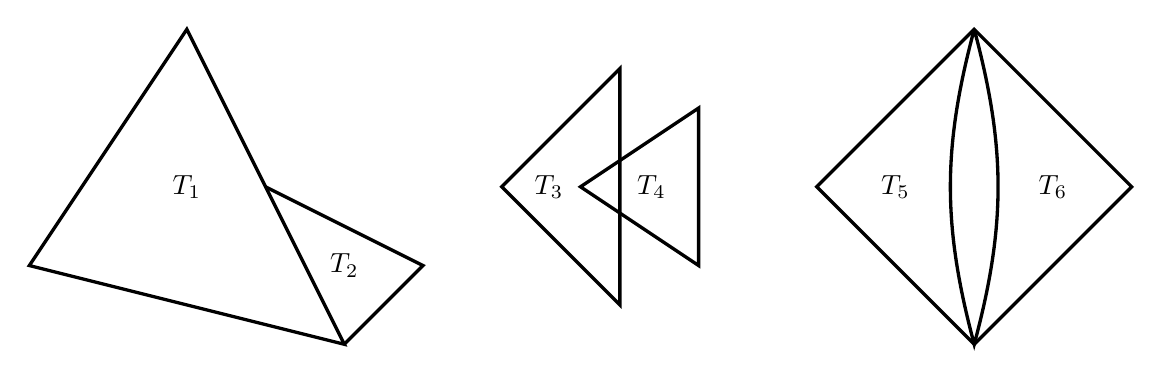
\begin{tikzpicture}
	\def \angle{15}
	\draw[very thick] (0, 0) -- (2, 3) -- (4, -1) -- cycle;
	\draw[very thick] (4, -1) -- (5, 0) -- (3, 1);
	%\\
	\draw[very thick] (6, 0+1) -- (7.5, 1.5+1) -- (7.5, -1.5+1) -- cycle;
	\draw[very thick] (7, 0+1) -- (8.5, 1+1) -- (8.5, -1+1) -- cycle;
	%
	\draw[very thick] (10, 1) -- (12, 3) -- (14, 1) -- (12, -1) -- cycle;
	\draw[very thick] (12, 3) to [out=270+\angle,in=90-\angle] (12, -1) to [out=90+\angle,in=270-\angle] (12, 3);
	\node[] at (2, 1)   (a) {$T_1$};
	\node[] at (4, 0)   (b) {$T_2$};
	\node[] at (6.6, 1)   (c) {$T_3$};
	\node[] at (7.9, 1)   (d) {$T_4$};
	\node[] at (11, 1)   (a) {$T_5$};
	\node[] at (13, 1)   (a) {$T_6$};
\end{tikzpicture}
  \caption{Some types of intersections \emph{forbidden} in a triangulation.}
  \label{fig:triang unallowed}
\end{figure}
Given any compact surface $S,$ it seems plausible that there should exist a triangulation of $S.$ It is indeed the case, as was proven by T. Radó. Proving this is \emph{not} trivial but we will take this for granted.\\
We can regard a triangulated surface as having been constructed by gluing together the various triangles in a certain way, much as we put together a jigsaw puzzle. As two different triangles cannot have the same vertices, we can specify completely a triangulation of a surface by numbering the vertices, and then listing which triples of vertices are vertices of a triangle. Such a list of triangles completely determines the surface together with the given triangulation up to homeomorphism.\\~\\
\textsc{Some Triangulations:}\\\\
1) The surface of an ordinary tetrahedron in $\mathbb{R}^3$ is homeomorphic to the sphere $S^2;$ moreover, the four triangles satisfy all the conditions for a triangulation of $S^2.$ In this case, there are four vertices, and every triple of vertices is the set of vertices of a triangle.\\\\
2) In Figure \ref{fig:pplane triang}, we show a triangulation of the projective plane, considered as the space obtained by identifying diametrically opposite points on the boundary of a disc. The vertices are numbered from $1$ to $6,$ and there are the following $10$ triangles:
\begin{center}
  $124$ \hfil $245$\\
  $235$ \hfil $135$\\
  $156$ \hfil $126$\\
  $236$ \hfil $346$\\
  $134$ \hfil $456$
\end{center}

\begin{figure}[!htb]
  \centering
  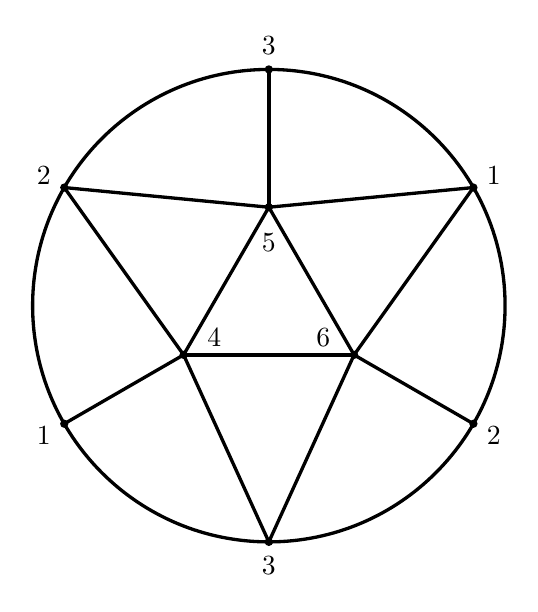
\begin{tikzpicture}
	\def \radius{3} % of circle
	\def \tri{1.25}
	\def \theta{pi/3}
	\def \dist{0.3}
	%triangle nodes
	\fill ({\tri*sin(( 0 *2*\theta) r)}, {\tri*cos(( 0 *2*\theta) r)}) circle (1.5pt);
	\fill ({\tri*sin(( 1 *2*\theta) r)}, {\tri*cos(( 1 *2*\theta) r)}) circle (1.5pt);
	\fill ({\tri*sin(( 2 *2*\theta) r)}, {\tri*cos(( 2 *2*\theta) r)}) circle (1.5pt);
	%circle nodes
	\fill ({\radius*sin(( 0 *\theta) r)}, {\radius*cos(( 0 *\theta) r)}) circle (1.5pt);
	\fill ({\radius*sin(( 1 *\theta) r)}, {\radius*cos(( 1 *\theta) r)}) circle (1.5pt);
	\fill ({\radius*sin(( 2 *\theta) r)}, {\radius*cos(( 2 *\theta) r)}) circle (1.5pt);
	\fill ({\radius*sin(( 3 *\theta) r)}, {\radius*cos(( 3 *\theta) r)}) circle (1.5pt);
	\fill ({\radius*sin(( 4 *\theta) r)}, {\radius*cos(( 4 *\theta) r)}) circle (1.5pt);
	\fill ({\radius*sin(( 5 *\theta) r)}, {\radius*cos(( 5 *\theta) r)}) circle (1.5pt);
	\draw[very thick] (0, 0) circle (\radius);
	%making lines
	\draw[very thick] ({\tri*sin(( 0 *2*\theta) r)}, {\tri*cos(( 0 *2*\theta) r)}) -- ({\radius*sin(( 5 *\theta) r)}, {\radius*cos(( 5 *\theta) r)});
	\draw[very thick] ({\tri*sin(( 0 *2*\theta) r)}, {\tri*cos(( 0 *2*\theta) r)}) -- ({\radius*sin(( 0 *\theta) r)}, {\radius*cos(( 0 *\theta) r)});
	\draw[very thick] ({\tri*sin(( 0 *2*\theta) r)}, {\tri*cos(( 0 *2*\theta) r)}) -- ({\radius*sin(( 1 *\theta) r)}, {\radius*cos(( 1 *\theta) r)});
	\draw[very thick] ({\tri*sin(( 0 *2*\theta) r)}, {\tri*cos(( 0 *2*\theta) r)}) -- ({\tri*sin(( 1 *2*\theta) r)}, {\tri*cos(( 1 *2*\theta) r)});
	\draw[very thick] ({\tri*sin(( 1 *2*\theta) r)}, {\tri*cos(( 1 *2*\theta) r)}) -- ({\radius*sin(( 1 *\theta) r)}, {\radius*cos(( 1 *\theta) r)});
	\draw[very thick] ({\tri*sin(( 1 *2*\theta) r)}, {\tri*cos(( 1 *2*\theta) r)}) -- ({\radius*sin(( 2 *\theta) r)}, {\radius*cos(( 2 *\theta) r)});
	\draw[very thick] ({\tri*sin(( 1 *2*\theta) r)}, {\tri*cos(( 1 *2*\theta) r)}) -- ({\radius*sin(( 3 *\theta) r)}, {\radius*cos(( 3 *\theta) r)});
	\draw[very thick] ({\tri*sin(( 1 *2*\theta) r)}, {\tri*cos(( 1 *2*\theta) r)}) -- ({\tri*sin(( 2 *2*\theta) r)}, {\tri*cos(( 2 *2*\theta) r)});
	\draw[very thick] ({\tri*sin(( 2 *2*\theta) r)}, {\tri*cos(( 2 *2*\theta) r)}) -- ({\radius*sin(( 3 *\theta) r)}, {\radius*cos(( 3 *\theta) r)});
	\draw[very thick] ({\tri*sin(( 2 *2*\theta) r)}, {\tri*cos(( 2 *2*\theta) r)}) -- ({\radius*sin(( 4 *\theta) r)}, {\radius*cos(( 4 *\theta) r)});
	\draw[very thick] ({\tri*sin(( 2 *2*\theta) r)}, {\tri*cos(( 2 *2*\theta) r)}) -- ({\radius*sin(( 5 *\theta) r)}, {\radius*cos(( 5 *\theta) r)});
	\draw[very thick] ({\tri*sin(( 2 *2*\theta) r)}, {\tri*cos(( 2 *2*\theta) r)}) -- ({\tri*sin(( 3 *2*\theta) r)}, {\tri*cos(( 3 *2*\theta) r)});
	% labelling circle
	\node[] at ({(\radius + \dist)*sin(( 1 *\theta) r)}, {(\radius + \dist)*cos(( 1 *\theta) r)}) {$ 1 $};
	\node[] at ({(\radius + \dist)*sin(( 2 *\theta) r)}, {(\radius + \dist)*cos(( 2 *\theta) r)}) {$ 2 $};
	\node[] at ({(\radius + \dist)*sin(( 3 *\theta) r)}, {(\radius + \dist)*cos(( 3 *\theta) r)}) {$ 3 $};
	\node[] at ({(\radius + \dist)*sin(( 4 *\theta) r)}, {(\radius + \dist)*cos(( 4 *\theta) r)}) {$ 1 $};
	\node[] at ({(\radius + \dist)*sin(( 5 *\theta) r)}, {(\radius + \dist)*cos(( 5 *\theta) r)}) {$ 2 $};
	\node[] at ({(\radius + \dist)*sin(( 6 *\theta) r)}, {(\radius + \dist)*cos(( 6 *\theta) r)}) {$ 3 $};
	% labelling triangle
	\node[] at ({(\tri - 1.5*\dist)*sin(( 2 *2*\theta) r)}, {(\tri - 1.5*\dist)*cos(( 2 *2*\theta) r)}) {$ 4 $};
	\node[] at ({(\tri - 1.5*\dist)*sin(( 0 *2*\theta) r)}, {(\tri - 1.5*\dist)*cos(( 0 *2*\theta) r)}) {$ 5 $};
	\node[] at ({(\tri - 1.5*\dist)*sin(( 1 *2*\theta) r)}, {(\tri - 1.5*\dist)*cos(( 1 *2*\theta) r)}) {$ 6 $};
\end{tikzpicture}
  \caption{A triangulation of the projective plane.}
  \label{fig:pplane triang}
\end{figure}

3) In Figure \ref{fig:torus triang}, we show a triangulation of a torus, regarded as a square with the opposite sides identified. There are $9$ vertices, and the following $18$ triangles:
\begin{center}
  $124$ \hfil $245$ \hfil $235$\\
  $356$ \hfil $361$ \hfil $146$\\
  $457$ \hfil $578$ \hfil $658$\\
  $689$ \hfil $649$ \hfil $479$\\
  $187$ \hfil $128$ \hfil $289$\\
  $239$ \hfil $379$ \hfil $137$\\
\end{center}

\begin{figure}[!htb]
  \centering
  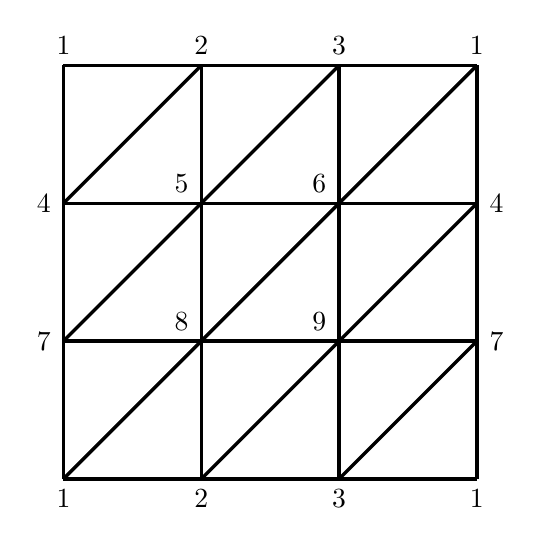
\begin{tikzpicture}
	\def \unit{1.75}
	\def \sep{0.25}
	\foreach \x in {0,1,...,3}{\draw[very thick] (\unit*\x, 0) -- (\unit*\x, 3*\unit);\draw[very thick] (0, \unit*\x) -- (3*\unit, \unit*\x);};
	\foreach \x in {0,1,...,2}{\draw[very thick] (0, \unit*\x) -- ({(3-\x)*\unit}, {3*\unit}); \draw[very thick] (\x*\unit, 0) -- ({3*\unit}, {(3-\x)*\unit});};
	% row 1
	\foreach \x in {1,2,...,3}{\node[] at ({(\x-1)*\unit}, 3*\unit+\sep) {$\x$};}; % top 1 2 3
	\node[] at (3*\unit, 3*\unit+\sep) {$1$};
	% row 2
	\node[] at (-\sep, 2*\unit) {$4$};
	\node[] at (\unit-\sep, 2*\unit+\sep) {$5$};
	\node[] at (2*\unit-\sep, 2*\unit+\sep) {$6$};
	\node[] at (3*\unit+\sep, 2*\unit) {$4$};
	% row 3
	\node[] at (-\sep, \unit) {$7$};
	\node[] at (\unit-\sep, \unit+\sep) {$8$};
	\node[] at (2*\unit-\sep, \unit+\sep) {$9$};
	\node[] at (3*\unit+\sep, \unit) {$7$};
	% row 4
	\foreach \x in {1,2,...,3}{\node[] at ({(\x-1)*\unit}, -\sep) {$\x$};}; % bottom 1 2 3
	\node[] at (3*\unit, -\sep) {$1$};
\end{tikzpicture}
  \caption{A triangulation of a torus.}
  \label{fig:torus triang}
\end{figure}
We conclude our discussion of triangulations by noting that any triangulation of a compact surface $S$ satisfies the following two conditions:
\begin{enumerate}[nosep, label = (\arabic*)] 
  \item Each edge is an edge of exactly two triangles.
  \item Let $v$ be a vertex of a triangulation. Then we may arrange the set of all triangles with $v$ as a vertex in cyclic order, $T_0,\; T_1,\; \cdots,\; T_{n-1},\; T_n = T_0,$ such that $T_i$ and $T_{i+1}$ have an edge in common for $0 \le i \le n-1.$
\end{enumerate}
The truth of (1) follows from the fact that each point on the edge in question must have an open neighbourhood homeomorphic to the open disc $B^2.$ If an edge were an edge of only one triangle or more than two triangles, this would not be possible. The rigorous proof of this last assertion can be given using the concept of ``The local homology groups at a point." We will omit this.\\
Condition (2) can be demonstrated as follows.\\
Given $v,$ let us define two triangles $A_i$ and $A_j$ having $v$ as a vertex to be \emph{equivalent} if there is a sequence of triangles having $v$ as a vertex, beginning with $A_i$ and ending with $A_j,$ such that the intersection of each triangle with its successor is an edge of each. If there is more than one equivalence class, let $B$ be the union of the triangles in one class and $C$ be the union of the others. The sets $B$ and $C$ intersect in $v$ alone because no triangle in $B$ has an edge common with a triangle in $C.$ We conclude that \emph{for every sufficiently small neighbourhood $W$ of $v$ in $X$, the space $W-\{v\}$ is not connected.}\\
On the other hand, if $S$ is a surface, then $v$ has a neighbourhood homeomorphic to $B^2.$ In this case, $v$ has arbitrarily small neighbourhoods $W$ such that $W - \{v\}$ is connected (Lemma \ref{lem:connected balls}), a contradiction.\\
Thus, we have shown that since $S$ is a surface, a situation such as that indicated in Figure \ref{fig:triang vertex} cannot happen.

\begin{figure}[!htb]
  \centering
  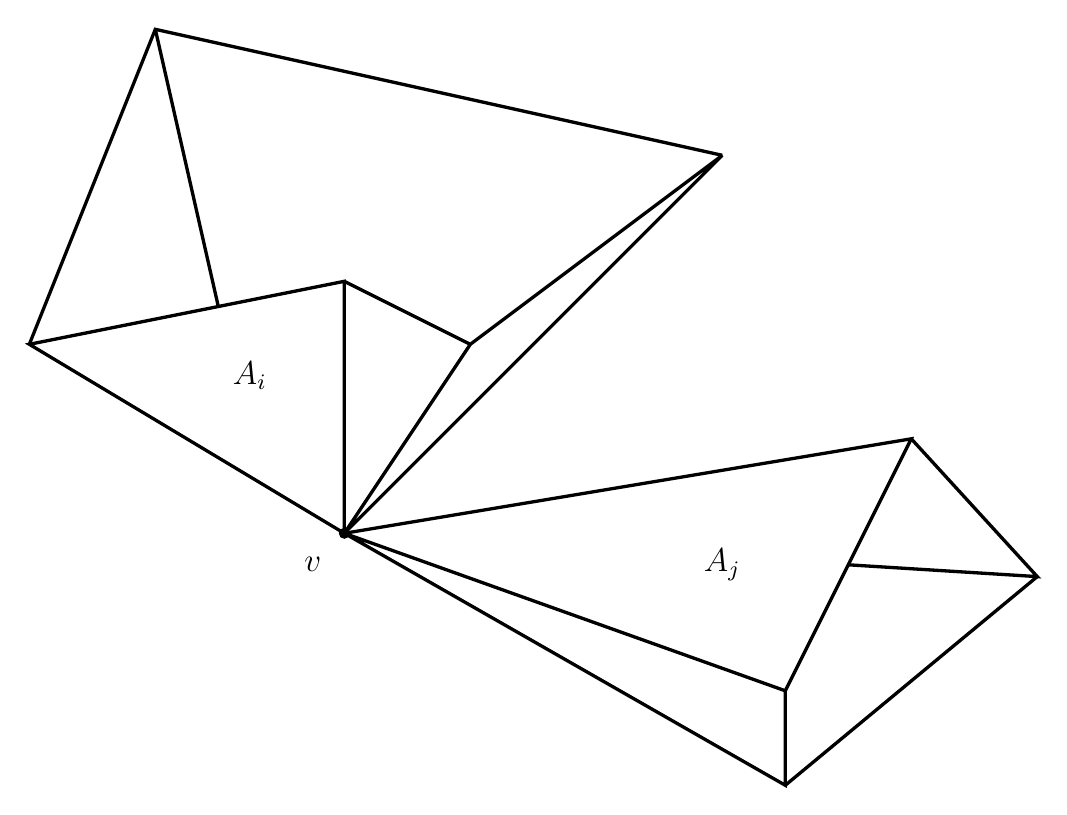
\begin{tikzpicture}[scale=0.8]
	\coordinate (a) at (0, 0);
	\coordinate (b) at (2, 3);
	\coordinate (c) at (6, 6);
	\coordinate (d) at (0, 4);
	\coordinate (e) at (-5, 3);
	\coordinate (f) at (-3, 8);
	\coordinate (g) at (-2, 18/5);
	\draw[very thick] (a) -- (b) -- (c) -- cycle;
	\draw[very thick] (a) -- (e) -- (d) -- cycle;
	\draw[very thick] (d) -- (b);
	\draw[very thick] (f) -- (g);
	\draw[very thick] (e) -- (f) -- (c);
	%
	\coordinate (h) at (7, -4);
	\coordinate (i) at (7, -2.5);
	\coordinate (j) at (9, 1.5);
	\coordinate (k) at (11, -11/16);
	\coordinate (l) at (8, -.5);	
	\draw[very thick] (a) -- (i) -- (h) -- cycle;
	\draw[very thick] (a) -- (j) -- (i);
	\draw[very thick] (j) -- (k) -- (l);
	\draw[very thick] (k) -- (h);
	%
	\fill (a) circle (2.5pt);
	\node[] at (-1.5, 2.5) {\begin{large}$A_i$\end{large}};
	\node[] at (6, -0.5) {\begin{large}$A_j$\end{large}};
	\node[] at (-0.5, -0.5) {\begin{large}$v$\end{large}};
\end{tikzpicture}
  \caption{Such a case is not possible.}
  \label{fig:triang vertex}
\end{figure}
%
\newpage
\section{A Surprising Lemma}
%
We will now state and prove a surprising lemma that will help us later.
\begin{lem}\label{lem:surprise}
  The connected sum of a torus and a projective plane is homeomorphic to the connected sum of three projective planes.
\end{lem}
\begin{proof}
$ $\newline
\begin{adjustwidth}{-20mm}{-20mm}
  \begin{center}
    \begin{tikzpicture}
	\draw[ultra thin] (-0.5, -2.5) rectangle (7, 2.5);
	\node[] at (-0.5+.25, -2.5+0.25) {\scriptsize (1)};
	\def \length{3}
	\def \sep{0.5}
	\def \theta{60} % in degrees
	

	\draw[thick, ->-=at 0.5 with label {\small $a$}] (0, 0) to [out=\theta, in=180-\theta] (\length, 0);
	\draw[thick, ->-=at 0.5 with label {\small $a$}] (\length, 0) to [out=180+\theta, in=360-\theta] (0, 0);
	\draw[thick, ->-=at 0.52 with label {\footnotesize $d$}, variable=\t,domain=pi/2:3*pi/2,samples=500] plot ({0.4*\length*cos((\t) r) + \length},{0.1*\length*sin((2*\t) r)});

	\def \length{1.5}

	\draw[thick, ->-=at 0.5 with label {\small $b$}] (2*\length + \sep,0) -- (3*\length + \sep, \length);
	\draw[thick, ->-=at 0.5 with label {\small $c$}] (3*\length + \sep, \length) -- (4*\length + \sep, 0);
	\draw[thick, -<-=at 0.5 with label {\small $b$}] (4*\length + \sep, 0) -- (3*\length + \sep, -\length);
	\draw[thick, -<-=at 0.5 with label {\small $c$}] (3*\length + \sep, -\length) -- (2*\length + \sep,0);
	  \draw[thick, -<-=at 0.5 with label {\footnotesize $d$}, variable=\t,domain=pi/2:3*pi/2,samples=500] plot ({-0.9*\length*cos((\t) r) + 2*\length + \sep},{-0.25*\length*sin((2*\t) r)});
\end{tikzpicture}
    \begin{tikzpicture}
	\draw[ultra thin] (-0.5, -2.5) rectangle (6, 2.5);
	\node[] at (-0.5+0.25, -2.5+0.25) {\scriptsize (2)};
	\def \length{2.5}
	\def \height{1}
	\def \sep{-0.6}
	\draw[thick, ->-=at 0.55 with label {\small $a$}] (0, 0) -- (\length, \height/2);
	\draw[thick, ->-=at 0.52 with label {\footnotesize $d$}] (\length, -\height/2) -- (\length, \height/2);
	\draw[thick, ->-=at 0.45 with label {\small $a$}] (\length, -\height/2) -- (0, 0);

	\def \length{1.5}
	
	 
	\draw[thick, -<-=at 0.5 with label {\footnotesize $d$}] (\length/3 + 2*\length + \sep, \length/3) -- (\length/3 + 2*\length + \sep, -\length/3);

	\draw[thick, ->-=at 0.5 with label {\small $b$}] (\length/3 + 2*\length + \sep, \length/3) -- (\length + 2*\length + \sep, \length);
	\draw[thick, ->-=at 0.5 with label {\small $c$}] (\length + 2*\length + \sep, \length) -- (2*\length+2*\length+\sep, 0);
	\draw[thick, -<-=at 0.5 with label {\small $b$}] (2*\length+2*\length+\sep, 0) -- (\length + 2*\length + \sep, -\length);
	\draw[thick, -<-=at 0.5 with label {\small $c$}] (\length + 2*\length + \sep, -\length) -- (\length/3 + 2*\length + \sep, -\length/3);
\end{tikzpicture}

    \begin{tikzpicture}
	\draw[ultra thin] (-2.5, -2.5) rectangle (2.5, 2.5);
	\node[] at (-2.5 + 0.25, -2.5 + 0.25) {\scriptsize (3)};
	\def \x {0}
	\def \y {0}
	\def \radius {2}	
	\draw[thick, ->-=at 0.5 with label {$a$}] 
												({\x - \radius*cos((0 * pi/3) r)}, {\y + \radius*sin((0 * pi/3) r)}) -- 
												({\x - \radius*cos((1 * pi/3) r)}, {\y + \radius*sin((1 * pi/3) r)});
	\draw[thick, ->-=at 0.5 with label {$b$}] 
												({\x - \radius*cos((1 * pi/3) r)}, {\y + \radius*sin((1 * pi/3) r)}) -- 
												({\x - \radius*cos((2 * pi/3) r)}, {\y + \radius*sin((2 * pi/3) r)});
	\draw[thick, ->-=at 0.5 with label {$c$}] 
												({\x - \radius*cos((2 * pi/3) r)}, {\y + \radius*sin((2 * pi/3) r)}) -- 
												({\x - \radius*cos((3 * pi/3) r)}, {\y + \radius*sin((3 * pi/3) r)});
	\draw[thick, -<-=at 0.5 with label {$b$}] 
												({\x - \radius*cos((3 * pi/3) r)}, {\y + \radius*sin((3 * pi/3) r)}) -- 
												({\x - \radius*cos((4 * pi/3) r)}, {\y + \radius*sin((4 * pi/3) r)});
	\draw[thick, -<-=at 0.5 with label {$c$}] 
												({\x - \radius*cos((4 * pi/3) r)}, {\y + \radius*sin((4 * pi/3) r)}) -- 
												({\x - \radius*cos((5 * pi/3) r)}, {\y + \radius*sin((5 * pi/3) r)});
	\draw[thick, ->-=at 0.5 with label {$a$}] 
												({\x - \radius*cos((5 * pi/3) r)}, {\y + \radius*sin((5 * pi/3) r)}) -- 
												({\x - \radius*cos((0 * pi/3) r)}, {\y + \radius*sin((0 * pi/3) r)});
\end{tikzpicture}
    \input{TikzFiles/Lemma-TP-PPP/TikzTP-PPP04.tex}
    \input{TikzFiles/Lemma-TP-PPP/TikzTP-PPP05.tex}

    \begin{tikzpicture}
	\draw[ultra thin] (-2.5, -2.5) rectangle (2.5, 2.5);
	\node[] at (-2.5 + 0.25, -2.5 + 0.25) {\scriptsize (6)};
	\def \wid {3} % smol width
	\def \height {4}
	\def \width {4.5} %big width
	\draw[thick, -<-=at 0.5 with label {$a$}] (-\wid/2, 0) -- (\wid/2, 0);
	\draw[thick, -<-=at 0.5 with label {$e$}] (\width/2, \height/2) -- (\wid/2, 0);
	\draw[thick, ->-=at 0.5 with label {$c$}] (-\width/2, \height/2) -- (\width/2, \height/2);
	\draw[thick, ->-=at 0.5 with label {$b$}] (-\wid/2, 0) -- (-\width/2, \height/2);

	\draw[thick, ->-=at 0.5 with label {$c$}] (\wid/2, 0) -- (\width/2, -\height/2);
	\draw[thick, ->-=at 0.5 with label {$b$}] (\width/2, -\height/2) -- (-\width/2, -\height/2);
	\draw[thick, -<-=at 0.5 with label {$e$}] (-\width/2, -\height/2) -- (-\wid/2, 0);
\end{tikzpicture}
    \input{TikzFiles/Lemma-TP-PPP/TikzTP-PPP07.tex}
    \input{TikzFiles/Lemma-TP-PPP/TikzTP-PPP08.tex}
  \end{center}

  \input{TikzFiles/Lemma-TP-PPP/TikzTP-PPP09.tex}
  \begin{tikzpicture}
	\def \x {0}
	\def \y {0}
	\def \radius {2}
	\def \del{0.5}
	\draw[ultra thin] (-2.5, -2.5) rectangle (2.5 +\del, 2.5);
	\node[] at (-2.5 + 0.26, -2.5 + 0.25) {\scriptsize (10)};
	\draw[thick, -<-=at 0.5 with label {$e$}] 
	({\x - \radius*cos((0 * pi/3) r)}, {\y + \radius*sin((0 * pi/3) r)}) -- 
	({\x - \radius*cos((1 * pi/3) r)}, {\y + \radius*sin((1 * pi/3) r)});
	\draw[thick, ->-=at 0.5 with label {$b$}] 
	({\x - \radius*cos((1 * pi/3) r)}, {\y + \radius*sin((1 * pi/3) r)}) -- 
	({\x - \radius*cos((2 * pi/3) r)}, {\y + \radius*sin((2 * pi/3) r)});
	\draw[thick, ->-=at 0.5 with label {$c$}] 
	({\x +\del - \radius*cos((2 * pi/3) r)}, {\y + \radius*sin((2 * pi/3) r)}) -- 
	({\x +\del - \radius*cos((3 * pi/3) r)}, {\y + \radius*sin((3 * pi/3) r)});
	\draw[thick, -<-=at 0.5 with label {$e$}] 
	({\x +\del - \radius*cos((3 * pi/3) r)}, {\y + \radius*sin((3 * pi/3) r)}) -- 
	({\x +\del - \radius*cos((4 * pi/3) r)}, {\y + \radius*sin((4 * pi/3) r)});
	\draw[thick, ->-=at 0.5 with label {$c$}] 
	({\x - \radius*cos((4 * pi/3) r)}, {\y + \radius*sin((4 * pi/3) r)}) -- 
	({\x - \radius*cos((5 * pi/3) r)}, {\y + \radius*sin((5 * pi/3) r)});
	\draw[thick, ->-=at 0.5 with label {$b$}] 
	({\x - \radius*cos((5 * pi/3) r)}, {\y + \radius*sin((5 * pi/3) r)}) -- 
	({\x - \radius*cos((0 * pi/3) r)}, {\y + \radius*sin((0 * pi/3) r)});


	\draw[thick, -<-=at 0.5 with label {$f$}] ({\x - \radius*cos((4 * pi/3) r)}, {\y + \radius*sin((4 * pi/3) r)}) -- ({\x - \radius*cos((2 * pi/3) r)}, {\y + \radius*sin((2 * pi/3) r)});
	\draw[thick, ->-=at 0.5 with label {$f$}] ({\x +\del - \radius*cos((2 * pi/3) r)}, {\y + \radius*sin((2 * pi/3) r)}) -- ({\x +\del - \radius*cos((4 * pi/3) r)}, {\y + \radius*sin((4 * pi/3) r)});
\end{tikzpicture}
  \input{TikzFiles/Lemma-TP-PPP/TikzTP-PPP11.tex}

  \begin{tikzpicture}
	\def \x {0}
	\def \y {0}
	\def \radius {2}
	\draw[ultra thin] (-2.5 -0.25, -2.5) rectangle (2.5 +0.25, 2.5);
	\node[] at (-2.5 + 0.25, -2.5 + 0.25) {\scriptsize (12)};
	\draw[thick, ->-=at 0.5 with label {$b$}] 
												({\x - \radius*cos((0 * pi/3) r)}, {\y + \radius*sin((0 * pi/3) r)}) -- 
												({\x - \radius*cos((1 * pi/3) r)}, {\y + \radius*sin((1 * pi/3) r)});
	\draw[thick, ->-=at 0.5 with label {$f$}] 
												({\x - \radius*cos((1 * pi/3) r)}, {\y + \radius*sin((1 * pi/3) r)}) -- 
												({\x - \radius*cos((2 * pi/3) r)}, {\y + \radius*sin((2 * pi/3) r)});
	\draw[thick, ->-=at 0.5 with label {$f$}] 
												({\x  - \radius*cos((2 * pi/3) r)}, {\y + \radius*sin((2 * pi/3) r)}) -- 
												({\x  - \radius*cos((3 * pi/3) r)}, {\y + \radius*sin((3 * pi/3) r)});
	\draw[thick, ->-=at 0.5 with label {$e$}] 
												({\x  - \radius*cos((3 * pi/3) r)}, {\y + \radius*sin((3 * pi/3) r)}) -- 
												({\x  - \radius*cos((4 * pi/3) r)}, {\y + \radius*sin((4 * pi/3) r)});
	\draw[thick, ->-=at 0.5 with label {$b$}] 
												({\x - \radius*cos((4 * pi/3) r)}, {\y + \radius*sin((4 * pi/3) r)}) -- 
												({\x - \radius*cos((5 * pi/3) r)}, {\y + \radius*sin((5 * pi/3) r)});
	\draw[thick, -<-=at 0.5 with label {$e$}] 
												({\x - \radius*cos((5 * pi/3) r)}, {\y + \radius*sin((5 * pi/3) r)}) -- 
												({\x - \radius*cos((0 * pi/3) r)}, {\y + \radius*sin((0 * pi/3) r)});


	\draw[thick, dashed, -<-=at 0.52 with label {$g$}] ({\x  - \radius*cos((1 * pi/3) r)}, {\y + \radius*sin((1 * pi/3) r)}) -- ({\x  - \radius*cos((5 * pi/3) r)}, {\y + \radius*sin((5 * pi/3) r)});
\end{tikzpicture}
  \input{TikzFiles/Lemma-TP-PPP/TikzTP-PPP13.tex}
  \input{TikzFiles/Lemma-TP-PPP/TikzTP-PPP14.tex}

  \begin{center}
    \input{TikzFiles/Lemma-TP-PPP/TikzTP-PPP15.tex}
  \end{center}
\end{adjustwidth}
$ $\newline
We start with a projective plane and a torus with holes cut in (1); using a series of cutting and gluing of edges, we arrive at (15), which represents the connected sum of three projective planes (see Figure \ref{fig:pplane 3 sum}). As all the diagrams represent homeomorphic surfaces, we have proven the lemma.\\~\\
\end{proof}
We now have all the preliminaries required for the proof of Theorem \ref{thm:main}.
%
\newpage
\section{Proof of The Theorem}
%
Let $S$ be a compact surface. We shall demonstrate Theorem \ref{thm:main} by proving that $S$ is homeomorphic to a polygon with the edges identified in pairs as indicated by one of the symbols listed at the end of Section \ref{sec:statement}.\\

\emph{First step.} From the discussion in the Section \ref{sec:triangulations}, we may assume that $S$ is triangulated. Denote the number of triangles by $n.$ We assert that we can number the triangles $T_1,\; T_2, \cdots,\; T_n,$ so that the triangle $T_i$ has an edge $e_i$ in common with at least one of the the triangles $T_1, \cdots,\; T_{i-1}$ for $2 \le i \le n.$ To prove this assertion, label any of the triangles $T_1;$ for $T_2$ choose any triangle that has an edge in common with $T_1,$ for $T_3$ choose any triangle that has an edge in common with $T_1$ or $T_2,$ et cetera. If at any stage we could not continue this process, then we would have two sets of triangles $\{T_1, \cdots,\; T_k\}$ and $\{T_{k+1}, \cdots,\; T_n\}$ such that no triangle in the first set would have an edge or vertex in common with any triangle of the second set. But this would give a partition of $S$ into two disjoint non-empty closed sets, contrary to the assumption that $S$ was connected.\\
We now use this ordering of triangles, $T_1,\;T_2,\;\cdots,\;T_n,$ together with the choice of edges $e_2,$ $e_3,$ $\cdots,$ $e_n,$ to construct a ``model'' of the the surface $S$ on the Euclidean plane; this model will be a polygon whose sides are to be identified in pairs. Recall that for each triangle $T_i,$ there exists an ordinary Euclidean triangle $T_i'$ in $\mathbb{R}^2$ and a homeomorphism $\varphi_i$ of $T_i'$ onto $T_i.$ We can assume that the triangles $T_1',\;T_2',\cdots,\;T_n'$ are pairwise disjoint; if they are not, we can translate some of them to various other parts of the plane $\mathbb{R}^2.$ Let
\[T' = \bigcup_{i=1}^nT_i';\]
then $T'$ is a compact subset of $\mathbb{R}^2.$ ($T'$ is a finite union of closed and bounded subsets and is thus, closed and bounded itself. Compactness follows from Theorem \ref{thm:heine-borel}.)\\
Define a map $\varphi:T'\longrightarrow S$ by $\varphi|T_i' = \varphi_i;$ the map $\varphi$ is obviously continuous and onto. As $T'$ is compact, any closed subset $A$ of $T'$ is compact (Theorem \ref{thm:compact closed}). Thus, $\varphi(A) \subset S$ is compact. As $S$ is a Hausdorff space, $\varphi(A)$ is closed (Theorem \ref{thm:compact haus}). Therefore, $\varphi$ is a closed map, and hence $S$ has the quotient topology induced by $\varphi$ (Lemma \ref{lem:closed maps quotient}).\\
This is a rigorous mathematical statement of out intuitive idea that $S$ is obtained by gluing the triangles $T_1,\;T_2,\;\cdots$ together along the appropriate edges.\\
The polygon we desire will be constructed as a quotient space of $T'.$ Consider any of the edges $e_i,\;2\le i \le n.$ By assumption, $e_i$ is a edge of the triangle $T_i$ and on other triangle $T_j,$ for which $1 \le j < i.$ Therefore $\varphi^{-1}(e_i)$ consists of an edge of the triangles $T_i'$ and $T_j'$ by identifying points which map onto the same point of $e_i.$ We make these identifications for each of the edges $e_2,\;e_3,\cdots,\;e_n.$ Let $D$ denote the resulting quotient space of $T'.$ It is clear that the map $\varphi:T' \longrightarrow S$ induces a map $\psi$ of $D$ onto $S.$ As $D$ is compact and $S$ Hausdorff, $\psi$ is a closed map. (By the same reasoning we used for $\varphi$.) Thus, $S$ has the quotient topology induced by $\psi.$\\
We now assert that topologically, $D$ is a closed disc. The proof depends on two facts:
\begin{enumerate}[label = (\alph*)] 
  \item Let $E_1$ and $E_2$ be disjoint spaces, which topologically are closed disc (i.e., they are homeomorphic to $E^2$). Let $A_1$ and $A_2$ be subsets of the boundary of $E_1$ and $E_2,$ respectively, which are homeomorphic to the closed interval $[0, 1],$ and let $h:A_1 \longrightarrow A_2$ be a definite homeomorphism. Form a quotient space of $E_1 \cup E_2$ by identifying points that correspond under $h.$ Then, topologically, the quotient space is also a closed disc.\\
  This can be demonstrated as follows. Given $E_1$ and $A_1,$ we can find a homeomorphism $h_1$ such that $h_1$ maps $E_1$ to a closed unit square $S_1$ and $A_1$ to one of its edges. We can similarly map $E_2$ to a square $S_2$ and $A_2$ to one of its edge. Now, we identify the edges of the squares. It can be easily seen that this quotient space is homeomorphic to a closed rectangle that is twice as long as it is wide. This rectangle is, in turn, homeomorphic to $E^2.$
  \item  In forming the quotient space $D$ of $T',$ we may either make all the identifications at once, or make the identifications corresponding to $e_2,$ then those corresponding to $e_3,$ et cetera, in succession. This can shown by using induction and the fact that $e_i \neq e_j$ if $i \neq j.$
\end{enumerate}
We now use these facts to prove that $D$ is a disc as follows. $T_1'$ and $T_2'$ are topologically equivalent to discs. Therefore, the quotient space of $T_1' \cup T_2'$ obtained by identifying points of $\varphi^{-1}(e_2)$ is again a disc by (a). Form a quotient space of this disc and $T_3'$ by making the identifications corresponding to the edge $e_3,$ et cetera.\\
It is clear that $S$ is obtained from $D$ by identifying certain paired edges on the boundary of $D$.\\~\\
\emph{Second step. Elimination of adjacent edges of the first kind.} We have now obtained a polygon $D$ whose edges have to be identified in pairs to obtain the given surface $S.$ These identifications may be indicated by the appropriate symbol.\\
If the letter designating a certain pair of edges occurs with \emph{both} exponents $+1$ and $-1,$ in the symbol, then we will call that pair of edges a pair of \emph{first kind;} otherwise, the pair is of the \emph{second kind.} \\
We wish to show that an adjacent pair of edges of the first kind be eliminated, provided there are at least four edges in all. This is easily seen from the sequence of diagrams in Figure \ref{fig:step two}. We can continue this process until all such pairs are eliminated, or until we obtain a polygon with only two sides. In the latter case, this polygon, whose symbol will be $aa$ or $aa^{-1},$ must be a projective plane or a sphere, and we have completed the proof. Otherwise, we must continue as follows.\\

\begin{figure}[!htb]
  \centering
  \begin{tikzpicture}
	\coordinate (a) at (-1.5, -2);
	\coordinate (b) at (-1, -0.75);
	\coordinate (c) at (0, 0);
	\coordinate (d) at (1, -0.75);
	\coordinate (e) at (1.5, -2);
	\draw[very thick] (a) -- (b);
	\draw[very thick,->-=at 0.5 with label {$a$}] (b) -- (c);
	\draw[very thick,-<-=at 0.5 with label {$a$}] (c) -- (d);
	\draw[very thick] (d) -- (e);
	\draw [very thick, decorate, decoration=snake, segment amplitude=.6mm, segment length=2mm] (a) to [out=300, in=240] (e);
 	\fill (a) circle (2pt);
 	\fill (b) circle (2pt);
 	\fill (c) circle (2pt);
 	\fill (d) circle (2pt);
 	\fill (e) circle (2pt);
 	%
 	\coordinate (a) at (-1.5+5, -2);
	\coordinate (b) at (-0.9+5, -0);
	\coordinate (c) at (0+5, -1);
	\coordinate (d) at (0.9+5, -0);
	\coordinate (e) at (1.5+5, -2);
	\draw[very thick] (a) -- (b);
	\draw[very thick,->-=at 0.5 with label {\small $a$}] (b) -- (c);
	\draw[very thick,-<-=at 0.5 with label {\small $a$}] (c) -- (d);
	\draw[very thick] (d) -- (e);
	\draw [very thick, decorate, decoration=snake, segment amplitude=.6mm, segment length=2mm] (a) to [out=300, in=240] (e);
 	\fill (a) circle (2pt);
 	\fill (b) circle (2pt);
 	\fill (c) circle (2pt);
 	\fill (d) circle (2pt);
 	\fill (e) circle (2pt);
 	%
	\coordinate (a) at (-1.75, -1 -4.75);
	\coordinate (b) at (-0.2, -0 -4.75);
	\coordinate (c) at (0, -1.5 -4.75);
	\coordinate (d) at (0.2, -0 -4.75);
	\coordinate (e) at (1.75, -1 -4.75);
	\draw[very thick] (a) -- (b);
	\draw[very thick,-<-=at 0.5 with label {$a$}] (c) -- (b);
	\draw[very thick,->-=at 0.5 with label {$a$}] (d) -- (c);
	\draw[very thick] (d) -- (e);
	\draw [very thick, decorate, decoration=snake, segment amplitude=.6mm, segment length=2mm] (a) .. controls (-1.7, -4 -4.75) and (1.7, -4 -4.75) .. (e);
 	\fill (a) circle (2pt);
 	\fill (b) circle (2pt);
 	\fill (c) circle (2pt);
 	\fill (d) circle (2pt);
 	\fill (e) circle (2pt);
 	%
	\coordinate (a) at (-1.75 +5, -1 -4.75);
	\coordinate (b) at (0 +5, -0 -4.75);
	\coordinate (c) at (0 +5, -1.5 -4.75);
	\coordinate (e) at (1.75 +5, -1 -4.75);
	\draw[very thick] (a) -- (b);
	\draw[very thick,-<-=at 0.5 with label {$a$}] (c) -- (b);
	\draw[very thick] (b) -- (e);
	\draw [very thick, decorate, decoration=snake, segment amplitude=.6mm, segment length=2mm] (a) .. controls (-1.7 +5, -4 -4.75) and (1.7 +5, -4 -4.75) .. (e);
 	\fill (a) circle (2pt);
 	\fill (b) circle (2pt);
 	\fill (c) circle (2pt);
 	\fill (e) circle (2pt);
 	\node[] at (0, -3.25) {(a)};
 	\node[] at (5, -3.25) {(b)};
 	\node[] at (0, -3.25 -5.25) {(c)};
 	\node[] at (5, -3.25 -5.25) {(d)};
\end{tikzpicture}
  \caption{Elimination of an adjacent pair of edges of the first kind.}
  \label{fig:step two}
\end{figure}
\emph{Third step. Transformation to a polygon such that all vertices must be identified to a single vertex.} Although the edges of our polygon must be identified in pairs, the vertices may be identified in sets of one, two, three, et cetera. Let us call two vertices of the polygon \emph{equivalent} if and only if they are to be identified. Some equivalence classes contain only one vertex, whereas other classes contain two or three.\\
Assume we have carried out step two as far as possible. We wish to prove that we can transform our polygon into another polygon with all its vertices belonging to one equivalence class.

\begin{figure}[!htb]
  \centering
  \begin{tikzpicture}
	\coordinate (a) at (-1.5, -1.2);
	\coordinate (b) at (0, 0);
	\coordinate (c) at (1.5, -1.2);
	\coordinate (d) at (-1.5, -4);
	\coordinate (e) at (1.5, -4);
	\draw[very thick, ->-=at 0.5 with label {$a$}] (a) -- (b);
	\draw[very thick, -<-=at 0.5 with label {$b$}] (b) -- (c);
	\draw[very thick, -<-=at 0.5 with label {$c$}] (c) -- (a);
	\draw[very thick, -<-=at 0.5 with label {$a$}] (e) -- (d);
	\draw [very thick, decorate, decoration=snake, segment amplitude=.6mm, segment length=2mm] (a) to [out=240, in=120] (d);
	\draw [very thick, decorate, decoration=snake, segment amplitude=.6mm, segment length=2mm] (c) to [out=300, in=60] (e);
 	\fill (a) circle (2pt);
 	\fill (b) circle (2pt);
 	\fill (c) circle (2pt);
 	\fill (d) circle (2pt);
 	\fill (e) circle (2pt);
 	%
 	\coordinate (a) at (-1.5 +5.0, -1.2);
	\coordinate (b) at (0 +5.0, -5.5);
	\coordinate (c) at (1.5 +5.0, -1.2);
	\coordinate (d) at (-1.5 +5.0, -4);
	\coordinate (e) at (1.5 +5.0, -4);
	\draw[very thick, -<-=at 0.5 with label {$c$}] (b) -- (d);
	\draw[very thick, -<-=at 0.5 with label {$b$}] (e) -- (b);
	\draw[very thick, -<-=at 0.5 with label {$c$}] (c) -- (a);
	\draw[very thick, -<-=at 0.5 with label {$a$}] (e) -- (d);
	\draw [very thick, decorate, decoration=snake, segment amplitude=.6mm, segment length=2mm] (a) to [out=240, in=120] (d);
	\draw [very thick, decorate, decoration=snake, segment amplitude=.6mm, segment length=2mm] (c) to [out=300, in=60] (e);
 	\fill (a) circle (2pt);
 	\fill (b) circle (2pt);
 	\fill (c) circle (2pt);
 	\fill (d) circle (2pt);
 	\fill (e) circle (2pt);
 	%
 	\node [] at (0, 0.5) {$P$};
 	\node [] at (1.6, -0.9) {$Q$};
 	\node [] at (-1.6, -0.9) {$R$};
 	\node [] at (1.6 +5.0, -0.9) {$R$};
 	\node [] at (-1.6 +5.0, -0.9) {$Q$};
 	\node [] at (1.6, -4.25) {$P$};
 	\node [] at (-1.6, -4.25) {$R$};
 	\node [] at (1.6 +5.0, -4.25) {$P$};
 	\node [] at (-1.6 +5.0, -4.25) {$R$};
 	\node [] at (0.4 +5.0, -5.5) {$Q$};
 	%
 	\node[] at (0, -6) {(a)};
 	\node[] at (0 +5.0, -6) {(b)};
\end{tikzpicture}
  \caption{Third step in the proof.}
  \label{fig:step three}
\end{figure}
Suppose there are at least two different equivalence classes of vertices. Then, the polygon must have an adjacent pair of vertices which are non-equivalent. Label these vertices $P$ and $Q.$ Figure \ref{fig:step three} shows how to proceed. As $P$ and $Q$ are non-equivalent, and we have carried out step two, it follows that sides $a$ and $b$ are \emph{not} to be identified. Make a cut along the line labeled $c,$ from the vertex labeled $Q$ to the other vertex of the edge (i.e., to the vertex of edge $a$ which is distinct from $P$). Then, glue the two edges labeled $a$ together. A new polygon with one less vertex in the equivalence class of $P$ and one more vertex in the equivalence class of $Q$ results. If possible, perform step two again. Then carry out step three to reduce the vertices in the equivalence class of $P$ still further, then do step two again. Continue alternately doing step three and step two until the equivalence class of $P$ is eliminated entirely. If more than one equivalence class of vertices remains, we can repeat this procedure to reduce the number by $1.$ If we continue in this manner, we ultimately obtain a polygon such that all the vertices are to be identified to a single vertex.\\~\\
%
\emph{Fourth step. How to make any pair of edges of the second kind adjacent.} We wish to show that our surface can be transformed so that any pair of edges of the second kind are adjacent to each other. Suppose we have a pair of edges of the second kind which are non-adjacent, as in Figure \ref{fig:step four}(a). Cut along the dotted line labeled $a$ and paste together along $b.$ As shown in Figure \ref{fig:step four}(b), the two edges are now adjacent. Also, note that all adjacent pairs of edges that don't include $b$ are not affected. 

\begin{figure}[!htb]
  \centering
  \begin{tikzpicture}
	\coordinate (a) at (-1, -0.5);
	\coordinate (b) at (-1.75, -1.75);
	\coordinate (c) at (1, -0.5);
	\coordinate (d) at (1.75, -1.75);
	\draw[very thick, -<-=at 0.5 with label {$b$}] (b) -- (a);
	\draw[very thick, -<-=at 0.5 with label {$b$}] (c) -- (d);
	\draw[very thick, decorate, decoration=snake, segment amplitude=.6mm, segment length=1.5mm] (a) to [out=30,in=150] (c);
	\draw[very thick, decorate, decoration=snake, segment amplitude=.6mm, segment length=1.5mm] (b) to [out=300,in=240] (d);
	\draw[very thick, dashed, ->-=at 0.5 with label {$a$}] (c) -- (b);
 	\fill (a) circle (2pt);
 	\fill (b) circle (2pt);
 	\fill (c) circle (2pt);
 	\fill (d) circle (2pt);
	%
	\coordinate (a) at (-1 +5.0, -0.75);
	\coordinate (b) at (0 +5.0, 0);
	\coordinate (c) at (1 +5.0, -0.75);
	\coordinate (d) at (0 +5.0, -2.5);
	\draw[very thick, -<-=at 0.5 with label {$a$}] (a) -- (b);
	\draw[very thick, -<-=at 0.5 with label {$a$}] (b) -- (c);
	\draw[very thick, decorate, decoration=snake, segment amplitude=.6mm, segment length=1.5mm] (a) .. controls (-1.25 +5.0, -2) .. (d) .. controls (1.25 +5.0, -2) .. (c);
	%\draw[very thick, decorate, decoration=snake, segment amplitude=.6mm, segment length=1.5mm] (c) .. controls (1 +5.0, -2) .. (d);
	\draw[very thick, dashed, ->-=at 0.5 with label {$b$}] (d) -- (b);
 	\fill (a) circle (2pt);
 	\fill (b) circle (2pt);
 	\fill (c) circle (2pt);
 	\fill (d) circle (2pt);
	%
	\node[] at (0, -3.5) {(a)};
	\node[] at (0 +5.0, -3.5) {(b)};
\end{tikzpicture}
  \caption{Fourth step in the proof.}
  \label{fig:step four}
\end{figure}
\begin{figure}[!htb]
  \centering
  \begin{tikzpicture}
	\coordinate (a) at (-1.5, 0.75);
	\coordinate (b) at (-1.5, -0.75);
	\coordinate (c) at (1.5, 0.75);
	\coordinate (d) at (1.5, -0.75);
	\draw[very thick, ->-=at 0.5 with label {$c$}] (b) -- (a);
	\draw[very thick, -<-=at 0.5 with label {$c$}] (c) -- (d);
	\draw[very thick, decorate, decoration=snake, segment amplitude=.6mm, segment length=1.5mm] (a) to [out=60,in=120] (c);
	\draw[very thick, decorate, decoration=snake, segment amplitude=.6mm, segment length=1.5mm] (b) to [out=300,in=240] (d);
 	\fill (a) circle (2pt);
 	\fill (b) circle (2pt);
 	\fill (c) circle (2pt);
 	\fill (d) circle (2pt);
 	\node[] at (0, 2) {$A$};
 	\node[] at (0, -2) {$B$};
\end{tikzpicture}
  \caption{A pair of edges of the first kind.}
  \label{fig:step four-2}
\end{figure}
Continue this process until all pairs of edges of the second kind are adjacent. If there are no pairs of the first kind, we are finished, because the symbol of the polygon must then be of the form $a_1a_1a_2a_2\cdots a_na_n,$ and hence $S$ is the connected sum of $n$ projective planes.\\
Assume to the contrary that at this stage there is at least one pair of edges of the first kind, each of which is labeled with the letter $c.$ Then we assert that there is at least one other pair of edges of the first kind such that these two pairs separate one another; i.e., edges from two pairs occur alternately as we proceed around the boundary of the polygon (hence, the symbol must be of the form $c\ldots d \ldots c^{-1} \ldots d^{-1},$ where the dots denote the possible occurrence of other letters).\\
To prove this assertion, assume that the edges labeled $c$ are not separated by any other pair of the first kind. Then our polygon has the appearance indicated in Figure \ref{fig:step four-2}. Here $A$ and $B$ designate a whole sequence of edges. The important point is that any edge in $A$ must be identified another edge in $A,$ and similarly for $B$. (This is because all the pairs of second kind are adjacent and we have assumed that no pair of first kind is separating the pair of edges labeled $c$). Thus, no edge in $A$ is to be identified with an edge in $B.$ Let the vertex connecting $c$ to $A$ be labeled $P.$ All the vertices in $A$ must be identified with $P$ as $A$ consists of adjacent pairs of the second kind. As no edge of $A$ is identified with any end of $B$ and neither are the starting points of edge $c,$ the vertices of $B$ must not be identified with $P.$ This contradicts our activity of Step 3.\\~\\
%
\emph{Fifth step. Pairs of the first kind.} Suppose, then, that we have two pairs of the first kind which separate each other as described (see Figure \ref{fig:step five} (a)). We shall show that we can transform the polygon so that the four sides in question are consecutive around the perimeter of the polygon.

\begin{figure}[!htb]
  \centering
  \begin{tikzpicture}
	\coordinate (a) at (-1.5, 0.75);
	\coordinate (b) at (-1.5, -0.75);
	\coordinate (c) at (1.5, 0.75);
	\coordinate (d) at (1.5, -0.75);

	\coordinate (e) at (-1, 2);
	\coordinate (f) at (1, 2);
	\coordinate (g) at (-1, -1.75);
	\coordinate (h) at (1, -1.75);

	\draw[very thick, ->-=at 0.5 with label {$a$}] (b) -- (a);
	\draw[very thick, -<-=at 0.5 with label {$a$}] (c) -- (d);
	\draw[very thick, ->-=at 0.5 with label {$b$}] (e) -- (f);
	\draw[very thick, -<-=at 0.5 with label {$b$}] (h) -- (g);
	\draw[very thick, dashed, ->-=at 0.5 with label {$c$}] (c) -- (a);
	\draw[very thick, decorate, decoration=snake, segment amplitude=.6mm, segment length=1.75mm] (a) -- (e);
	\draw[very thick, decorate, decoration=snake, segment amplitude=.6mm, segment length=1.75mm] (f) -- (c);
	\draw[very thick, decorate, decoration=snake, segment amplitude=.6mm, segment length=1.75mm] (b) -- (g);
	\draw[very thick, decorate, decoration=snake, segment amplitude=.6mm, segment length=1.75mm] (d) -- (h);
 	\fill (a) circle (2pt);
 	\fill (b) circle (2pt);
 	\fill (c) circle (2pt);
 	\fill (d) circle (2pt);
 	\fill (e) circle (2pt);
 	\fill (f) circle (2pt);
 	\fill (g) circle (2pt);
 	\fill (h) circle (2pt);
 	% (b)
 	\coordinate (a) at (-2 +6.0, 0.75);
	\coordinate (b) at (-1.85 +6.0, -0.75);
	\coordinate (c) at (2 +6.0, 0.75);
	\coordinate (d) at (1.85 +6.0, -0.75);

	\coordinate (e) at (-1.25 +6.0, 2);
	\coordinate (f) at (1.25 +6.0, 2);
	\coordinate (g) at (-1.25 +6.0, -1.75);
	\coordinate (h) at (1.25 +6.0, -1.75);

	\draw[very thick, decorate, decoration=snake, segment amplitude=.6mm, segment length=1.75mm] (b) -- (a);
	\draw[very thick, decorate, decoration=snake, segment amplitude=.6mm, segment length=1.75mm] (c) -- (d);
	\draw[very thick, -<-=at 0.5 with label {$c$}] (e) -- (f);
	\draw[very thick, ->-=at 0.5 with label {$c$}] (h) -- (g);
	\draw[very thick, dashed, ->-=at 0.5 with label {$b$}] (b) -- (d);
	\draw[very thick, ->-=at 0.5 with label {$a$}] (a) -- (e);
	\draw[very thick, -<-=at 0.5 with label {$a$}] (f) -- (c);
	\draw[very thick, decorate, decoration=snake, segment amplitude=.6mm, segment length=1.75mm] (b) -- (g);
	\draw[very thick, decorate, decoration=snake, segment amplitude=.6mm, segment length=1.75mm] (d) -- (h);
 	\fill (a) circle (2pt);
 	\fill (b) circle (2pt);
 	\fill (c) circle (2pt);
 	\fill (d) circle (2pt);
 	\fill (e) circle (2pt);
 	\fill (f) circle (2pt);
 	\fill (g) circle (2pt);
 	\fill (h) circle (2pt);
 	% (c)
 	\coordinate (a) at (-2, 0.75 -6.0);
	\coordinate (b) at (-1.85, -0.75 -6.0);
	\coordinate (c) at (2, 0.75 -6.0);
	\coordinate (d) at (1.85, -0.75 -6.0);

	\coordinate (e) at (-1.25, 2 -6.0);
	\coordinate (f) at (1.25, 2 -6.0);
	\coordinate (g) at (-1.25, -1.75 -6.0);
	\coordinate (h) at (1.25, -1.75 -6.0);

	\draw[very thick, decorate, decoration=snake, segment amplitude=.6mm, segment length=1.75mm] (b) -- (a);
	\draw[very thick, decorate, decoration=snake, segment amplitude=.6mm, segment length=1.75mm] (c) -- (d);
	\draw[very thick, -<-=at 0.5 with label {$c$}] (e) -- (f);
	\draw[very thick, ->-=at 0.5 with label {$c$}] (h) -- (g);
	\draw[very thick, dashed, -<-=at 0.5 with label {$d$}] (e) -- (g);
	\draw[very thick, ->-=at 0.5 with label {$a$}] (a) -- (e);
	\draw[very thick, -<-=at 0.5 with label {$a$}] (f) -- (c);
	\draw[very thick, decorate, decoration=snake, segment amplitude=.6mm, segment length=1.75mm] (b) -- (g);
	\draw[very thick, decorate, decoration=snake, segment amplitude=.6mm, segment length=1.75mm] (d) -- (h);
 	\fill (a) circle (2pt);
 	\fill (b) circle (2pt);
 	\fill (c) circle (2pt);
 	\fill (d) circle (2pt);
 	\fill (e) circle (2pt);
 	\fill (f) circle (2pt);
 	\fill (g) circle (2pt);
 	\fill (h) circle (2pt);
 	%(d)
 	\coordinate (a) at (-2 +6.0, 0.75 -6.0);
	\coordinate (b) at (-1.85 +6.0, -0.75 -6.0);
	\coordinate (c) at (2 +6.0, 0.75 -6.0);
	\coordinate (d) at (1.85 +6.0, -0.75 -6.0);

	\coordinate (e) at (-1.25 +6.0, 2 -6.0);
	\coordinate (f) at (1.25 +6.0, 2 -6.0);
	\coordinate (g) at (-1.25 +6.0, -1.75 -6.0);
	\coordinate (h) at (1.25 +6.0, -1.75 -6.0);

	\draw[very thick, ->-=at 0.5 with label {$d$}] (b) -- (a);
	\draw[very thick, decorate, decoration=snake, segment amplitude=.6mm, segment length=1.75mm] (c) -- (d);
	\draw[very thick, -<-=at 0.5 with label {$d$}] (e) -- (f);
	\draw[very thick, decorate, decoration=snake, segment amplitude=.6mm, segment length=1.75mm] (h) -- (g);
	\draw[very thick, dashed, -<-=at 0.5 with label {$a$}] (e) -- (d);
	\draw[very thick, -<-=at 0.5 with label {$c$}] (a) -- (e);
	\draw[very thick, decorate, decoration=snake, segment amplitude=.6mm, segment length=1.75mm] (f) -- (c);
	\draw[very thick, ->-=at 0.5 with label {$c$}] (g) -- (b);
	\draw[very thick, decorate, decoration=snake, segment amplitude=.6mm, segment length=1.75mm] (d) -- (h);
 	\fill (a) circle (2pt);
 	\fill (b) circle (2pt);
 	\fill (c) circle (2pt);
 	\fill (d) circle (2pt);
 	\fill (e) circle (2pt);
 	\fill (f) circle (2pt);
 	\fill (g) circle (2pt);
 	\fill (h) circle (2pt);
 	%
 	\node[] at (0, -2.6) {(a)};
 	\node[] at (0 +6.0, -2.6) {(b)};
 	\node[] at (0, -2.6 -6.0) {(b)};
 	\node[] at (0 +6.0, -2.6 -6.0) {(c)};
\end{tikzpicture}
  \caption{Fifth step in the proof.}
  \label{fig:step five}
\end{figure}
First, cut along $c$ and paste together along $b$ to obtained Figure \ref{fig:step five}(b). Then cut along $d$ and paste together along $a$ to obtain Figure \ref{fig:step five}(c), as desired.\\
Continue this process until all pairs of the first kind are in adjacent groups of four, as $cdc^{-1}d^{-1}$ in Figure \ref{fig:step five}(c). If there are no pairs of the second kind, this leads to the desired result because, in that case, the symbol must be of the form
\[a_1b_1a_1^{-1}b^{-1}a_2b_2a_2^{-1}b_2^{-1}\cdots a_nb_na_n^{-1}b_n^{-1}\]
and the surface is the connected sum of $n$ tori.\\~\\
%
\emph{Sixth step.} It remains to treat the case in which there are pairs of both the first and second kind at this stage. The key to this situation is lemma \ref{lem:surprise} from earlier. Assume that after the fifth step has been completed, the polygon has $m$ pairs ($m > 0$) of the second kind sch that the two edges of each pair are adjacent, and $n$ quadruples ($n > 0$) of sides, each quadruple consisting of two pairs of the first kind which separate each other. Then, the surface is the connected sum of $m$ projective planes and $n$ tori, which by the lemma is homeomorphic to the connected sum of $m + 2n$ projective planes. This completes the proof of Theorem \ref{thm:main}. \hfill $\blacksquare$
%
\section{The Euler Characteristic of a Surface}
%
Although we have shown that any compact surface is homeomorphic to a sphere, a sum of tori, or a sum of projective planes, we do not know that all these are topologically different. For example, it could be the case that there exist positive integers $m$ and $n$ with $m \neq n$ such that the sum of $m$ tori is homeomorphic to the sum of $n$ tori.\\
It can be shown that this is not the case with the help of a numerical invariant called the \emph{Euler characteristic}.\\
First, we define the Euler characteristic of a triangulated surface. Let $M$ be a compact surface with triangulation $\{T_1,\;\cdots,\;T_n\}.$ Let
\begin{center}
  $v = $ total number of vertices of $M,$\\
  $e = $ total number of edges of $M,$\\
  $f = $ total number of triangles (in this case, $t = n$).
\end{center}
Then,
\[\chi(M) = v - e + f\]
is called the \emph{Euler characteristic} of $M.$\\
It turns out that this number is independent of the way we choose to triangulate $M.$ Moreover, it can be shown that if $M$ and $N$ are homeomorphic, then $\chi(M) = \chi(N).$
\begin{lem}
  Let $S_1$ and $S_2$ be compact surfaces. The Euler characteristics of $S_1$ and $S_2$ and their connected sum, $S_1 \# S_2,$ are related by the formula 
  \[\chi(S_1 \# S_2) = \chi(S_1) + \chi(S_2) - 2.\]
\end{lem}
\begin{proof}
  Assume $S_1$ and $S_2$ are triangulated. Form their connected sum by removing from each the interior of a triangle, and then identifying edges and vertices of the boundaries of the removed triangles. The formula then follows by counting vertices, edges, and triangles before and after the formation of connected sum.
\end{proof}
From the triangulations of the sphere, torus and projective plane done before, we know their Euler characteristics. Using the above lemma and an obvious induction, we obtain the following values for the Euler characteristics.
\begin{center}
  \begin{tabular}{l c}
  \textbf{\emph{Surface}} & \textbf{\emph{Euler characteristic}} \\
  Sphere & $2$ \\
  Connected sum of $n$ tori & $2 - 2n$ \\
  Connected sum of $n$ projective planes & $2 - n$ \\
  \end{tabular}
\end{center}
The only case of overlap of Euler characteristics is that $\chi(nT^2) = \chi(2nP^2)$ where $nT^2$ is the connected sum of $n$ tori and $2nP^2$ is the connected sum of $2n$ projective planes. However, we observe that $nT^2$ is orientable whereas $2nP^2$ is not as it contains a M\"{o}bius strip.  \\\\
Assuming the topological invariance of the Euler characteristic and Theorem \ref{thm:main}, we have the following result:
\begin{theorem}
  Let $S_1$ and $S_2$ be compact surfaces. Then, $S_1$ and $S_2$ are homeomorphic if and only if their Euler characteristics are equal are both are orientable or both are non-orientable.
\end{theorem}

%
\addcontentsline{toc}{section}{References}
\bibliography{References}
\bibliographystyle{ieeetr}
\end{document}